\documentclass[1p]{elsarticle_modified}
%\bibliographystyle{elsarticle-num}

%\usepackage[colorlinks]{hyperref}
%\usepackage{abbrmath_seonhwa} %\Abb, \Ascr, \Acal ,\Abf, \Afrak
\usepackage{amsfonts}
\usepackage{amssymb}
\usepackage{amsmath}
\usepackage{amsthm}
\usepackage{scalefnt}
\usepackage{amsbsy}
\usepackage{kotex}
\usepackage{caption}
\usepackage{subfig}
\usepackage{color}
\usepackage{graphicx}
\usepackage{xcolor} %% white, black, red, green, blue, cyan, magenta, yellow
\usepackage{float}
\usepackage{setspace}
\usepackage{hyperref}

\usepackage{tikz}
\usetikzlibrary{arrows}

\usepackage{multirow}
\usepackage{array} % fixed length table
\usepackage{hhline}

%%%%%%%%%%%%%%%%%%%%%
\makeatletter
\renewcommand*\env@matrix[1][\arraystretch]{%
	\edef\arraystretch{#1}%
	\hskip -\arraycolsep
	\let\@ifnextchar\new@ifnextchar
	\array{*\c@MaxMatrixCols c}}
\makeatother %https://tex.stackexchange.com/questions/14071/how-can-i-increase-the-line-spacing-in-a-matrix
%%%%%%%%%%%%%%%

\usepackage[normalem]{ulem}

\newcommand{\msout}[1]{\ifmmode\text{\sout{\ensuremath{#1}}}\else\sout{#1}\fi}
%SOURCE: \msout is \stkout macro in https://tex.stackexchange.com/questions/20609/strikeout-in-math-mode

\newcommand{\cancel}[1]{
	\ifmmode
	{\color{red}\msout{#1}}
	\else
	{\color{red}\sout{#1}}
	\fi
}

\newcommand{\add}[1]{
	{\color{blue}\uwave{#1}}
}

\newcommand{\replace}[2]{
	\ifmmode
	{\color{red}\msout{#1}}{\color{blue}\uwave{#2}}
	\else
	{\color{red}\sout{#1}}{\color{blue}\uwave{#2}}
	\fi
}

\newcommand{\Sol}{\mathcal{S}} %segment
\newcommand{\D}{D} %diagram
\newcommand{\A}{\mathcal{A}} %arc


%%%%%%%%%%%%%%%%%%%%%%%%%%%%%5 test

\def\sl{\operatorname{\textup{SL}}(2,\Cbb)}
\def\psl{\operatorname{\textup{PSL}}(2,\Cbb)}
\def\quan{\mkern 1mu \triangleright \mkern 1mu}

\theoremstyle{definition}
\newtheorem{thm}{Theorem}[section]
\newtheorem{prop}[thm]{Proposition}
\newtheorem{lem}[thm]{Lemma}
\newtheorem{ques}[thm]{Question}
\newtheorem{cor}[thm]{Corollary}
\newtheorem{defn}[thm]{Definition}
\newtheorem{exam}[thm]{Example}
\newtheorem{rmk}[thm]{Remark}
\newtheorem{alg}[thm]{Algorithm}

\newcommand{\I}{\sqrt{-1}}
\begin{document}

%\begin{frontmatter}
%
%\title{Boundary parabolic representations of knots up to 8 crossings}
%
%%% Group authors per affiliation:
%\author{Yunhi Cho} 
%\address{Department of Mathematics, University of Seoul, Seoul, Korea}
%\ead{yhcho@uos.ac.kr}
%
%
%\author{Seonhwa Kim} %\fnref{s_kim}}
%\address{Center for Geometry and Physics, Institute for Basic Science, Pohang, 37673, Korea}
%\ead{ryeona17@ibs.re.kr}
%
%\author{Hyuk Kim}
%\address{Department of Mathematical Sciences, Seoul National University, Seoul 08826, Korea}
%\ead{hyukkim@snu.ac.kr}
%
%\author{Seokbeom Yoon}
%\address{Department of Mathematical Sciences, Seoul National University, Seoul, 08826,  Korea}
%\ead{sbyoon15@snu.ac.kr}
%
%\begin{abstract}
%We find all boundary parabolic representation of knots up to 8 crossings.
%
%\end{abstract}
%\begin{keyword}
%    \MSC[2010] 57M25 
%\end{keyword}
%
%\end{frontmatter}

%\linenumbers
%\tableofcontents
%
\newcommand\colored[1]{\textcolor{white}{\rule[-0.35ex]{0.8em}{1.4ex}}\kern-0.8em\color{red} #1}%
%\newcommand\colored[1]{\textcolor{white}{ #1}\kern-2.17ex	\textcolor{white}{ #1}\kern-1.81ex	\textcolor{white}{ #1}\kern-2.15ex\color{red}#1	}

{\Large $\underline{12a_{1070}~(K12a_{1070})}$}

\setlength{\tabcolsep}{10pt}
\renewcommand{\arraystretch}{1.6}
\vspace{1cm}\begin{tabular}{m{100pt}>{\centering\arraybackslash}m{274pt}}
\multirow{5}{120pt}{
	\centering
	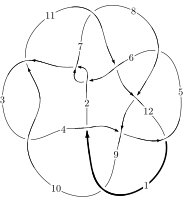
\includegraphics[width=112pt]{../../../GIT/diagram.site/Diagrams/png/1871_12a_1070.png}\\
\ \ \ A knot diagram\footnotemark}&
\allowdisplaybreaks
\textbf{Linearized knot diagam} \\
\cline{2-2}
 &
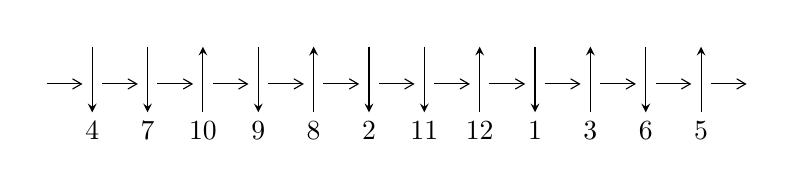
\begin{tikzpicture}[x=20pt, y=17pt]
	% nodes
	\node (C0) at (0, 0) {};
	\node (C1) at (1, 0) {};
	\node (C1U) at (1, +1) {};
	\node (C1D) at (1, -1) {4};

	\node (C2) at (2, 0) {};
	\node (C2U) at (2, +1) {};
	\node (C2D) at (2, -1) {7};

	\node (C3) at (3, 0) {};
	\node (C3U) at (3, +1) {};
	\node (C3D) at (3, -1) {10};

	\node (C4) at (4, 0) {};
	\node (C4U) at (4, +1) {};
	\node (C4D) at (4, -1) {9};

	\node (C5) at (5, 0) {};
	\node (C5U) at (5, +1) {};
	\node (C5D) at (5, -1) {8};

	\node (C6) at (6, 0) {};
	\node (C6U) at (6, +1) {};
	\node (C6D) at (6, -1) {2};

	\node (C7) at (7, 0) {};
	\node (C7U) at (7, +1) {};
	\node (C7D) at (7, -1) {11};

	\node (C8) at (8, 0) {};
	\node (C8U) at (8, +1) {};
	\node (C8D) at (8, -1) {12};

	\node (C9) at (9, 0) {};
	\node (C9U) at (9, +1) {};
	\node (C9D) at (9, -1) {1};

	\node (C10) at (10, 0) {};
	\node (C10U) at (10, +1) {};
	\node (C10D) at (10, -1) {3};

	\node (C11) at (11, 0) {};
	\node (C11U) at (11, +1) {};
	\node (C11D) at (11, -1) {6};

	\node (C12) at (12, 0) {};
	\node (C12U) at (12, +1) {};
	\node (C12D) at (12, -1) {5};
	\node (C13) at (13, 0) {};

	% arrows
	\draw[->,>={angle 60}]
	(C0) edge (C1) (C1) edge (C2) (C2) edge (C3) (C3) edge (C4) (C4) edge (C5) (C5) edge (C6) (C6) edge (C7) (C7) edge (C8) (C8) edge (C9) (C9) edge (C10) (C10) edge (C11) (C11) edge (C12) (C12) edge (C13) ;	\draw[->,>=stealth]
	(C1U) edge (C1D) (C2U) edge (C2D) (C3D) edge (C3U) (C4U) edge (C4D) (C5D) edge (C5U) (C6U) edge (C6D) (C7U) edge (C7D) (C8D) edge (C8U) (C9U) edge (C9D) (C10D) edge (C10U) (C11U) edge (C11D) (C12D) edge (C12U) ;
	\end{tikzpicture} \\
\hhline{~~} \\& 
\textbf{Solving Sequence} \\ \cline{2-2} 
 &
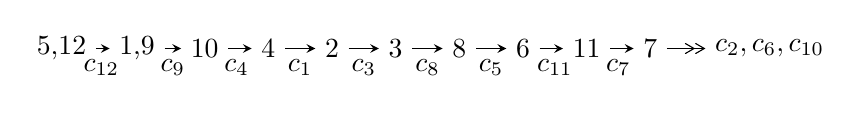
\begin{tikzpicture}[x=23pt, y=7pt]
	% node
	\node (A0) at (-1/8, 0) {5,12};
	\node (A1) at (17/16, 0) {1,9};
	\node (A2) at (17/8, 0) {10};
	\node (A3) at (25/8, 0) {4};
	\node (A4) at (33/8, 0) {2};
	\node (A5) at (41/8, 0) {3};
	\node (A6) at (49/8, 0) {8};
	\node (A7) at (57/8, 0) {6};
	\node (A8) at (65/8, 0) {11};
	\node (A9) at (73/8, 0) {7};
	\node (C1) at (1/2, -1) {$c_{12}$};
	\node (C2) at (13/8, -1) {$c_{9}$};
	\node (C3) at (21/8, -1) {$c_{4}$};
	\node (C4) at (29/8, -1) {$c_{1}$};
	\node (C5) at (37/8, -1) {$c_{3}$};
	\node (C6) at (45/8, -1) {$c_{8}$};
	\node (C7) at (53/8, -1) {$c_{5}$};
	\node (C8) at (61/8, -1) {$c_{11}$};
	\node (C9) at (69/8, -1) {$c_{7}$};
	\node (A10) at (11, 0) {$c_{2},c_{6},c_{10}$};

	% edge
	\draw[->,>=stealth]	
	(A0) edge (A1) (A1) edge (A2) (A2) edge (A3) (A3) edge (A4) (A4) edge (A5) (A5) edge (A6) (A6) edge (A7) (A7) edge (A8) (A8) edge (A9) ;
	\draw[->>,>={angle 60}]	
	(A9) edge (A10);
\end{tikzpicture} \\ 

\end{tabular} \\

\footnotetext{
The image of knot diagram is generated by the software ``\textbf{Draw programme}" developed by Andrew Bartholomew(\url{http://www.layer8.co.uk/maths/draw/index.htm\#Running-draw}), where we modified some parts for our purpose(\url{https://github.com/CATsTAILs/LinksPainter}).
}\phantom \\ \newline 
\centering \textbf{Ideals for irreducible components\footnotemark of $X_{\text{par}}$} 
 
\begin{align*}
I^u_{1}&=\langle 
9.45965\times10^{1721} u^{173}-4.57206\times10^{1722} u^{172}+\cdots+2.43243\times10^{1723} b+4.21326\times10^{1726},\\
\phantom{I^u_{1}}&\phantom{= \langle  }1.64927\times10^{1727} u^{173}-7.76624\times10^{1727} u^{172}+\cdots+2.70790\times10^{1728} a+9.82920\times10^{1731},\\
\phantom{I^u_{1}}&\phantom{= \langle  }u^{174}-5 u^{173}+\cdots+99447 u+22265\rangle \\
I^u_{2}&=\langle 
2.19598\times10^{92} u^{42}+4.98103\times10^{91} u^{41}+\cdots+3.59193\times10^{92} b+1.33922\times10^{93},\\
\phantom{I^u_{2}}&\phantom{= \langle  }4.87821\times10^{93} u^{42}+1.67362\times10^{92} u^{41}+\cdots+8.97983\times10^{93} a+8.06880\times10^{94},\;u^{43}+3 u^{40}+\cdots+29 u-5\rangle \\
\\
\end{align*}
\raggedright * 2 irreducible components of $\dim_{\mathbb{C}}=0$, with total 217 representations.\\
\footnotetext{All coefficients of polynomials are rational numbers. But the coefficients are sometimes approximated in decimal forms when there is not enough margin.}
\newpage
\renewcommand{\arraystretch}{1}
\centering \section*{I. $I^u_{1}= \langle 9.46\times10^{1721} u^{173}-4.57\times10^{1722} u^{172}+\cdots+2.43\times10^{1723} b+4.21\times10^{1726},\;1.65\times10^{1727} u^{173}-7.77\times10^{1727} u^{172}+\cdots+2.71\times10^{1728} a+9.83\times10^{1731},\;u^{174}-5 u^{173}+\cdots+99447 u+22265 \rangle$}
\flushleft \textbf{(i) Arc colorings}\\
\begin{tabular}{m{7pt} m{180pt} m{7pt} m{180pt} }
\flushright $a_{5}=$&$\begin{pmatrix}0\\u\end{pmatrix}$ \\
\flushright $a_{12}=$&$\begin{pmatrix}1\\0\end{pmatrix}$ \\
\flushright $a_{1}=$&$\begin{pmatrix}1\\- u^2\end{pmatrix}$ \\
\flushright $a_{9}=$&$\begin{pmatrix}-0.0609059 u^{173}+0.286799 u^{172}+\cdots-21655.1 u-3629.83\\-0.0388898 u^{173}+0.187963 u^{172}+\cdots-10866.0 u-1732.12\end{pmatrix}$ \\
\flushright $a_{10}=$&$\begin{pmatrix}-0.0335835 u^{173}+0.154766 u^{172}+\cdots-13908.3 u-2292.47\\-0.0332061 u^{173}+0.159047 u^{172}+\cdots-9802.45 u-1630.20\end{pmatrix}$ \\
\flushright $a_{4}=$&$\begin{pmatrix}-0.0989110 u^{173}+0.523817 u^{172}+\cdots-6895.26 u+2195.35\\0.00602631 u^{173}-0.0328215 u^{172}+\cdots-493.733 u-342.048\end{pmatrix}$ \\
\flushright $a_{2}=$&$\begin{pmatrix}-0.0158777 u^{173}-0.0132227 u^{172}+\cdots-45517.5 u-13549.2\\0.0248900 u^{173}-0.119614 u^{172}+\cdots+8107.31 u+1055.68\end{pmatrix}$ \\
\flushright $a_{3}=$&$\begin{pmatrix}-0.0960320 u^{173}+0.506440 u^{172}+\cdots-6276.04 u+2568.70\\-0.0544938 u^{173}+0.296688 u^{172}+\cdots-722.281 u+1762.03\end{pmatrix}$ \\
\flushright $a_{8}=$&$\begin{pmatrix}-0.0220161 u^{173}+0.0988365 u^{172}+\cdots-10789.1 u-1897.71\\-0.0388898 u^{173}+0.187963 u^{172}+\cdots-10866.0 u-1732.12\end{pmatrix}$ \\
\flushright $a_{6}=$&$\begin{pmatrix}-0.0777198 u^{173}+0.407364 u^{172}+\cdots-6627.03 u+1548.23\\-0.0272175 u^{173}+0.149275 u^{172}+\cdots+227.501 u+989.161\end{pmatrix}$ \\
\flushright $a_{11}=$&$\begin{pmatrix}-0.0129804 u^{173}+0.0565859 u^{172}+\cdots-667.159 u-222.955\\0.0435563 u^{173}-0.174852 u^{172}+\cdots+26617.6 u+6102.75\end{pmatrix}$ \\
\flushright $a_{7}=$&$\begin{pmatrix}0.0113813 u^{173}-0.0221015 u^{172}+\cdots+20549.4 u+6441.65\\-0.0483948 u^{173}+0.274933 u^{172}+\cdots+3710.35 u+2959.34\end{pmatrix}$\\&\end{tabular}
\flushleft \textbf{(ii) Obstruction class $= -1$}\\~\\
\flushleft \textbf{(iii) Cusp Shapes $= -0.103163 u^{173}+0.624534 u^{172}+\cdots+27015.3 u+11050.7$}\\~\\
\newpage\renewcommand{\arraystretch}{1}
\flushleft \textbf{(iv) u-Polynomials at the component}\newline \\
\begin{tabular}{m{50pt}|m{274pt}}
Crossings & \hspace{64pt}u-Polynomials at each crossing \\
\hline $$\begin{aligned}c_{1}\end{aligned}$$&$\begin{aligned}
&5(5 u^{174}-56 u^{173}+\cdots-31908 u+1387)
\end{aligned}$\\
\hline $$\begin{aligned}c_{2},c_{6}\end{aligned}$$&$\begin{aligned}
&u^{174}-2 u^{173}+\cdots+4042765 u+913579
\end{aligned}$\\
\hline $$\begin{aligned}c_{3},c_{10}\end{aligned}$$&$\begin{aligned}
&u^{174}+u^{173}+\cdots+131340 u+6023
\end{aligned}$\\
\hline $$\begin{aligned}c_{4}\end{aligned}$$&$\begin{aligned}
&5(5 u^{174}+26 u^{173}+\cdots+20363 u+1637)
\end{aligned}$\\
\hline $$\begin{aligned}c_{5}\end{aligned}$$&$\begin{aligned}
&5(5 u^{174}+86 u^{173}+\cdots+895002 u+151163)
\end{aligned}$\\
\hline $$\begin{aligned}c_{7}\end{aligned}$$&$\begin{aligned}
&5(5 u^{174}+43 u^{173}+\cdots-4.70613\times10^{9} u-3.70127\times10^{8})
\end{aligned}$\\
\hline $$\begin{aligned}c_{8}\end{aligned}$$&$\begin{aligned}
&u^{174}+4 u^{173}+\cdots-49199 u+15565
\end{aligned}$\\
\hline $$\begin{aligned}c_{9}\end{aligned}$$&$\begin{aligned}
&u^{174}+5 u^{173}+\cdots-1040129 u-102703
\end{aligned}$\\
\hline $$\begin{aligned}c_{11}\end{aligned}$$&$\begin{aligned}
&u^{174}- u^{173}+\cdots+18522 u+2029
\end{aligned}$\\
\hline $$\begin{aligned}c_{12}\end{aligned}$$&$\begin{aligned}
&u^{174}-5 u^{173}+\cdots+99447 u+22265
\end{aligned}$\\
\hline
\end{tabular}\\~\\
\newpage\renewcommand{\arraystretch}{1}
\flushleft \textbf{(v) Riley Polynomials at the component}\newline \\
\begin{tabular}{m{50pt}|m{274pt}}
Crossings & \hspace{64pt}Riley Polynomials at each crossing \\
\hline $$\begin{aligned}c_{1}\end{aligned}$$&$\begin{aligned}
&25(25 y^{174}-1136 y^{173}+\cdots-8.80288\times10^{7} y+1923769)
\end{aligned}$\\
\hline $$\begin{aligned}c_{2},c_{6}\end{aligned}$$&$\begin{aligned}
&y^{174}-114 y^{173}+\cdots-29118856544981 y+834626589241
\end{aligned}$\\
\hline $$\begin{aligned}c_{3},c_{10}\end{aligned}$$&$\begin{aligned}
&y^{174}+147 y^{173}+\cdots+21193565398 y+36276529
\end{aligned}$\\
\hline $$\begin{aligned}c_{4}\end{aligned}$$&$\begin{aligned}
&25(25 y^{174}+4 y^{173}+\cdots+1.13562\times10^{8} y+2679769)
\end{aligned}$\\
\hline $$\begin{aligned}c_{5}\end{aligned}$$&$\begin{aligned}
&25(25 y^{174}+304 y^{173}+\cdots-4.27927\times10^{11} y+2.28503\times10^{10})
\end{aligned}$\\
\hline $$\begin{aligned}c_{7}\end{aligned}$$&$\begin{aligned}
&25(25 y^{174}-1259 y^{173}+\cdots-7.99773\times10^{18} y+1.36994\times10^{17})
\end{aligned}$\\
\hline $$\begin{aligned}c_{8}\end{aligned}$$&$\begin{aligned}
&y^{174}-28 y^{173}+\cdots-20350176401 y+242269225
\end{aligned}$\\
\hline $$\begin{aligned}c_{9}\end{aligned}$$&$\begin{aligned}
&y^{174}-39 y^{173}+\cdots-2659529379217 y+10547906209
\end{aligned}$\\
\hline $$\begin{aligned}c_{11}\end{aligned}$$&$\begin{aligned}
&y^{174}+y^{173}+\cdots+126543508 y+4116841
\end{aligned}$\\
\hline $$\begin{aligned}c_{12}\end{aligned}$$&$\begin{aligned}
&y^{174}+27 y^{173}+\cdots+39776918751 y+495730225
\end{aligned}$\\
\hline
\end{tabular}\\~\\
\newpage\flushleft \textbf{(vi) Complex Volumes and Cusp Shapes}
$$\begin{array}{c|c|c}  
\text{Solutions to }I^u_{1}& \I (\text{vol} + \sqrt{-1}CS) & \text{Cusp shape}\\
 \hline 
\begin{aligned}
u &= -0.698557 + 0.698344 I \\
a &= \phantom{-}0.153713 - 0.930338 I \\
b &= \phantom{-}1.31046 - 0.91784 I\end{aligned}
 & \phantom{-}0.20315 - 4.84690 I & \phantom{-0.000000 } 0 \\ \hline\begin{aligned}
u &= -0.698557 - 0.698344 I \\
a &= \phantom{-}0.153713 + 0.930338 I \\
b &= \phantom{-}1.31046 + 0.91784 I\end{aligned}
 & \phantom{-}0.20315 + 4.84690 I & \phantom{-0.000000 } 0 \\ \hline\begin{aligned}
u &= \phantom{-}0.286593 + 0.975011 I \\
a &= \phantom{-}1.46215 + 0.51074 I \\
b &= \phantom{-}0.267939 - 0.084996 I\end{aligned}
 & -1.81985 - 1.82722 I & \phantom{-0.000000 } 0 \\ \hline\begin{aligned}
u &= \phantom{-}0.286593 - 0.975011 I \\
a &= \phantom{-}1.46215 - 0.51074 I \\
b &= \phantom{-}0.267939 + 0.084996 I\end{aligned}
 & -1.81985 + 1.82722 I & \phantom{-0.000000 } 0 \\ \hline\begin{aligned}
u &= -0.638165 + 0.744905 I \\
a &= -0.402101 + 0.324657 I \\
b &= -1.275630 + 0.347936 I\end{aligned}
 & \phantom{-}0.86953 + 2.10430 I & \phantom{-0.000000 } 0 \\ \hline\begin{aligned}
u &= -0.638165 - 0.744905 I \\
a &= -0.402101 - 0.324657 I \\
b &= -1.275630 - 0.347936 I\end{aligned}
 & \phantom{-}0.86953 - 2.10430 I & \phantom{-0.000000 } 0 \\ \hline\begin{aligned}
u &= \phantom{-}0.777829 + 0.677184 I \\
a &= \phantom{-}0.235396 + 0.509879 I \\
b &= \phantom{-}1.37533 + 1.01890 I\end{aligned}
 & -0.15603 + 6.59194 I & \phantom{-0.000000 } 0 \\ \hline\begin{aligned}
u &= \phantom{-}0.777829 - 0.677184 I \\
a &= \phantom{-}0.235396 - 0.509879 I \\
b &= \phantom{-}1.37533 - 1.01890 I\end{aligned}
 & -0.15603 - 6.59194 I & \phantom{-0.000000 } 0 \\ \hline\begin{aligned}
u &= \phantom{-}0.005088 + 0.961021 I \\
a &= -0.212205 + 0.093270 I \\
b &= -1.80034 + 0.14656 I\end{aligned}
 & -7.04267 + 0.20044 I & \phantom{-0.000000 } 0 \\ \hline\begin{aligned}
u &= \phantom{-}0.005088 - 0.961021 I \\
a &= -0.212205 - 0.093270 I \\
b &= -1.80034 - 0.14656 I\end{aligned}
 & -7.04267 - 0.20044 I & \phantom{-0.000000 } 0\\
 \hline 
 \end{array}$$\newpage$$\begin{array}{c|c|c}  
\text{Solutions to }I^u_{1}& \I (\text{vol} + \sqrt{-1}CS) & \text{Cusp shape}\\
 \hline 
\begin{aligned}
u &= -0.845850 + 0.450978 I \\
a &= \phantom{-}0.835697 + 0.397554 I \\
b &= -0.328803 + 0.365062 I\end{aligned}
 & -2.33913 + 0.17780 I & \phantom{-0.000000 } 0 \\ \hline\begin{aligned}
u &= -0.845850 - 0.450978 I \\
a &= \phantom{-}0.835697 - 0.397554 I \\
b &= -0.328803 - 0.365062 I\end{aligned}
 & -2.33913 - 0.17780 I & \phantom{-0.000000 } 0 \\ \hline\begin{aligned}
u &= \phantom{-}1.000410 + 0.312860 I \\
a &= -1.13257 + 0.90615 I \\
b &= \phantom{-}0.665417 + 0.372567 I\end{aligned}
 & -5.87512 + 0.12289 I & \phantom{-0.000000 } 0 \\ \hline\begin{aligned}
u &= \phantom{-}1.000410 - 0.312860 I \\
a &= -1.13257 - 0.90615 I \\
b &= \phantom{-}0.665417 - 0.372567 I\end{aligned}
 & -5.87512 - 0.12289 I & \phantom{-0.000000 } 0 \\ \hline\begin{aligned}
u &= \phantom{-}0.797274 + 0.682717 I \\
a &= \phantom{-}0.293997 + 0.663643 I \\
b &= \phantom{-}1.002460 + 0.711322 I\end{aligned}
 & \phantom{-}1.47877 + 2.36268 I & \phantom{-0.000000 } 0 \\ \hline\begin{aligned}
u &= \phantom{-}0.797274 - 0.682717 I \\
a &= \phantom{-}0.293997 - 0.663643 I \\
b &= \phantom{-}1.002460 - 0.711322 I\end{aligned}
 & \phantom{-}1.47877 - 2.36268 I & \phantom{-0.000000 } 0 \\ \hline\begin{aligned}
u &= \phantom{-}0.284471 + 0.905336 I \\
a &= -0.383310 - 0.450445 I \\
b &= -1.45671 - 0.43447 I\end{aligned}
 & \phantom{-}0.85549 + 3.26802 I & \phantom{-0.000000 } 0 \\ \hline\begin{aligned}
u &= \phantom{-}0.284471 - 0.905336 I \\
a &= -0.383310 + 0.450445 I \\
b &= -1.45671 + 0.43447 I\end{aligned}
 & \phantom{-}0.85549 - 3.26802 I & \phantom{-0.000000 } 0 \\ \hline\begin{aligned}
u &= -0.541287 + 0.766389 I \\
a &= \phantom{-}1.058720 - 0.937473 I \\
b &= \phantom{-}0.797198 + 0.116074 I\end{aligned}
 & -0.181454 + 0.443719 I & \phantom{-0.000000 } 0 \\ \hline\begin{aligned}
u &= -0.541287 - 0.766389 I \\
a &= \phantom{-}1.058720 + 0.937473 I \\
b &= \phantom{-}0.797198 - 0.116074 I\end{aligned}
 & -0.181454 - 0.443719 I & \phantom{-0.000000 } 0\\
 \hline 
 \end{array}$$\newpage$$\begin{array}{c|c|c}  
\text{Solutions to }I^u_{1}& \I (\text{vol} + \sqrt{-1}CS) & \text{Cusp shape}\\
 \hline 
\begin{aligned}
u &= -0.175493 + 1.056680 I \\
a &= -0.937739 - 0.770366 I \\
b &= \phantom{-}0.123094 - 0.880054 I\end{aligned}
 & -10.53250 - 4.51798 I & \phantom{-0.000000 } 0 \\ \hline\begin{aligned}
u &= -0.175493 - 1.056680 I \\
a &= -0.937739 + 0.770366 I \\
b &= \phantom{-}0.123094 + 0.880054 I\end{aligned}
 & -10.53250 + 4.51798 I & \phantom{-0.000000 } 0 \\ \hline\begin{aligned}
u &= \phantom{-}0.722774 + 0.575645 I \\
a &= \phantom{-}0.568934 + 0.744746 I \\
b &= \phantom{-}1.033990 + 0.137144 I\end{aligned}
 & \phantom{-}2.53301 + 2.01681 I & \phantom{-0.000000 } 0 \\ \hline\begin{aligned}
u &= \phantom{-}0.722774 - 0.575645 I \\
a &= \phantom{-}0.568934 - 0.744746 I \\
b &= \phantom{-}1.033990 - 0.137144 I\end{aligned}
 & \phantom{-}2.53301 - 2.01681 I & \phantom{-0.000000 } 0 \\ \hline\begin{aligned}
u &= -0.054555 + 1.097210 I \\
a &= -0.292802 + 0.882177 I \\
b &= \phantom{-}0.478007 + 0.899767 I\end{aligned}
 & -6.00326 + 0.51337 I & \phantom{-0.000000 } 0 \\ \hline\begin{aligned}
u &= -0.054555 - 1.097210 I \\
a &= -0.292802 - 0.882177 I \\
b &= \phantom{-}0.478007 - 0.899767 I\end{aligned}
 & -6.00326 - 0.51337 I & \phantom{-0.000000 } 0 \\ \hline\begin{aligned}
u &= -0.802357 + 0.764071 I \\
a &= -0.23165 + 1.39883 I \\
b &= -0.720143 + 0.315855 I\end{aligned}
 & \phantom{-}1.40094 - 7.28274 I & \phantom{-0.000000 } 0 \\ \hline\begin{aligned}
u &= -0.802357 - 0.764071 I \\
a &= -0.23165 - 1.39883 I \\
b &= -0.720143 - 0.315855 I\end{aligned}
 & \phantom{-}1.40094 + 7.28274 I & \phantom{-0.000000 } 0 \\ \hline\begin{aligned}
u &= -0.927107 + 0.607694 I \\
a &= \phantom{-}0.119337 - 0.431479 I \\
b &= \phantom{-}1.18174 - 0.80369 I\end{aligned}
 & \phantom{-}2.36415 - 2.87487 I & \phantom{-0.000000 } 0 \\ \hline\begin{aligned}
u &= -0.927107 - 0.607694 I \\
a &= \phantom{-}0.119337 + 0.431479 I \\
b &= \phantom{-}1.18174 + 0.80369 I\end{aligned}
 & \phantom{-}2.36415 + 2.87487 I & \phantom{-0.000000 } 0\\
 \hline 
 \end{array}$$\newpage$$\begin{array}{c|c|c}  
\text{Solutions to }I^u_{1}& \I (\text{vol} + \sqrt{-1}CS) & \text{Cusp shape}\\
 \hline 
\begin{aligned}
u &= \phantom{-}0.255798 + 0.831083 I \\
a &= \phantom{-}1.16903 + 1.15776 I \\
b &= \phantom{-}0.519313 + 0.654195 I\end{aligned}
 & -0.48095 + 2.13402 I & \phantom{-0.000000 } 0 \\ \hline\begin{aligned}
u &= \phantom{-}0.255798 - 0.831083 I \\
a &= \phantom{-}1.16903 - 1.15776 I \\
b &= \phantom{-}0.519313 - 0.654195 I\end{aligned}
 & -0.48095 - 2.13402 I & \phantom{-0.000000 } 0 \\ \hline\begin{aligned}
u &= -0.866531\phantom{ +0.000000I} \\
a &= \phantom{-}1.39589\phantom{ +0.000000I} \\
b &= -0.429024\phantom{ +0.000000I}\end{aligned}
 & -2.42565\phantom{ +0.000000I} & \phantom{-0.000000 } 0 \\ \hline\begin{aligned}
u &= \phantom{-}0.575877 + 0.646140 I \\
a &= \phantom{-}1.260670 + 0.598978 I \\
b &= \phantom{-}0.606518 - 0.366665 I\end{aligned}
 & -0.980758 - 0.917234 I & \phantom{-0.000000 } 0 \\ \hline\begin{aligned}
u &= \phantom{-}0.575877 - 0.646140 I \\
a &= \phantom{-}1.260670 - 0.598978 I \\
b &= \phantom{-}0.606518 + 0.366665 I\end{aligned}
 & -0.980758 + 0.917234 I & \phantom{-0.000000 } 0 \\ \hline\begin{aligned}
u &= -0.511372 + 0.695937 I \\
a &= \phantom{-}0.544200 - 1.206950 I \\
b &= \phantom{-}0.494477 + 0.045478 I\end{aligned}
 & \phantom{-}0.077511 + 0.797727 I & \phantom{-0.000000 } 0 \\ \hline\begin{aligned}
u &= -0.511372 - 0.695937 I \\
a &= \phantom{-}0.544200 + 1.206950 I \\
b &= \phantom{-}0.494477 - 0.045478 I\end{aligned}
 & \phantom{-}0.077511 - 0.797727 I & \phantom{-0.000000 } 0 \\ \hline\begin{aligned}
u &= \phantom{-}0.608205 + 0.961110 I \\
a &= \phantom{-}0.234990 + 1.299350 I \\
b &= \phantom{-}1.25675 + 1.42632 I\end{aligned}
 & -1.80993 + 5.69473 I & \phantom{-0.000000 } 0 \\ \hline\begin{aligned}
u &= \phantom{-}0.608205 - 0.961110 I \\
a &= \phantom{-}0.234990 - 1.299350 I \\
b &= \phantom{-}1.25675 - 1.42632 I\end{aligned}
 & -1.80993 - 5.69473 I & \phantom{-0.000000 } 0 \\ \hline\begin{aligned}
u &= -0.682883 + 0.912097 I \\
a &= \phantom{-}0.039149 - 1.117710 I \\
b &= \phantom{-}0.59356 - 1.45838 I\end{aligned}
 & -3.12491 - 5.02083 I & \phantom{-0.000000 } 0\\
 \hline 
 \end{array}$$\newpage$$\begin{array}{c|c|c}  
\text{Solutions to }I^u_{1}& \I (\text{vol} + \sqrt{-1}CS) & \text{Cusp shape}\\
 \hline 
\begin{aligned}
u &= -0.682883 - 0.912097 I \\
a &= \phantom{-}0.039149 + 1.117710 I \\
b &= \phantom{-}0.59356 + 1.45838 I\end{aligned}
 & -3.12491 + 5.02083 I & \phantom{-0.000000 } 0 \\ \hline\begin{aligned}
u &= -0.487179 + 1.042030 I \\
a &= \phantom{-}0.43495 - 1.39281 I \\
b &= \phantom{-}1.43063 - 1.26062 I\end{aligned}
 & -0.97011 - 4.47185 I & \phantom{-0.000000 } 0 \\ \hline\begin{aligned}
u &= -0.487179 - 1.042030 I \\
a &= \phantom{-}0.43495 + 1.39281 I \\
b &= \phantom{-}1.43063 + 1.26062 I\end{aligned}
 & -0.97011 + 4.47185 I & \phantom{-0.000000 } 0 \\ \hline\begin{aligned}
u &= \phantom{-}0.946470 + 0.668264 I \\
a &= -0.036513 - 1.150930 I \\
b &= -0.647454 - 0.150459 I\end{aligned}
 & \phantom{-}3.55036 + 2.34707 I & \phantom{-0.000000 } 0 \\ \hline\begin{aligned}
u &= \phantom{-}0.946470 - 0.668264 I \\
a &= -0.036513 + 1.150930 I \\
b &= -0.647454 + 0.150459 I\end{aligned}
 & \phantom{-}3.55036 - 2.34707 I & \phantom{-0.000000 } 0 \\ \hline\begin{aligned}
u &= -0.991020 + 0.602042 I \\
a &= -0.404303 + 0.294539 I \\
b &= -0.915098 + 0.090311 I\end{aligned}
 & \phantom{-}0.50080 + 2.53096 I & \phantom{-0.000000 } 0 \\ \hline\begin{aligned}
u &= -0.991020 - 0.602042 I \\
a &= -0.404303 - 0.294539 I \\
b &= -0.915098 - 0.090311 I\end{aligned}
 & \phantom{-}0.50080 - 2.53096 I & \phantom{-0.000000 } 0 \\ \hline\begin{aligned}
u &= -0.263831 + 0.782920 I \\
a &= \phantom{-}1.38228 + 0.84270 I \\
b &= -0.626392 + 0.696389 I\end{aligned}
 & -10.23540 - 0.95787 I & \phantom{-0.000000 } 0 \\ \hline\begin{aligned}
u &= -0.263831 - 0.782920 I \\
a &= \phantom{-}1.38228 - 0.84270 I \\
b &= -0.626392 - 0.696389 I\end{aligned}
 & -10.23540 + 0.95787 I & \phantom{-0.000000 } 0 \\ \hline\begin{aligned}
u &= \phantom{-}0.209122 + 0.797922 I \\
a &= -0.48023 - 1.47143 I \\
b &= \phantom{-}0.55463 - 1.56139 I\end{aligned}
 & -9.6261 + 12.1455 I & \phantom{-0.000000 } 0\\
 \hline 
 \end{array}$$\newpage$$\begin{array}{c|c|c}  
\text{Solutions to }I^u_{1}& \I (\text{vol} + \sqrt{-1}CS) & \text{Cusp shape}\\
 \hline 
\begin{aligned}
u &= \phantom{-}0.209122 - 0.797922 I \\
a &= -0.48023 + 1.47143 I \\
b &= \phantom{-}0.55463 + 1.56139 I\end{aligned}
 & -9.6261 - 12.1455 I & \phantom{-0.000000 } 0 \\ \hline\begin{aligned}
u &= -0.801321 + 0.175615 I \\
a &= \phantom{-}0.148585 + 1.339030 I \\
b &= -1.001470 + 0.261162 I\end{aligned}
 & -2.45495 - 5.46892 I & \phantom{-0.000000 } 0 \\ \hline\begin{aligned}
u &= -0.801321 - 0.175615 I \\
a &= \phantom{-}0.148585 - 1.339030 I \\
b &= -1.001470 - 0.261162 I\end{aligned}
 & -2.45495 + 5.46892 I & \phantom{-0.000000 } 0 \\ \hline\begin{aligned}
u &= \phantom{-}0.242934 + 1.156360 I \\
a &= \phantom{-}0.148743 - 0.648518 I \\
b &= \phantom{-}0.861747 - 0.849795 I\end{aligned}
 & -9.29684 + 4.33006 I & \phantom{-0.000000 } 0 \\ \hline\begin{aligned}
u &= \phantom{-}0.242934 - 1.156360 I \\
a &= \phantom{-}0.148743 + 0.648518 I \\
b &= \phantom{-}0.861747 + 0.849795 I\end{aligned}
 & -9.29684 - 4.33006 I & \phantom{-0.000000 } 0 \\ \hline\begin{aligned}
u &= -0.249608 + 0.770434 I \\
a &= -0.60933 + 1.39576 I \\
b &= \phantom{-}0.540275 + 1.237460 I\end{aligned}
 & -5.49891 - 6.54979 I & \phantom{-0.000000 } 0 \\ \hline\begin{aligned}
u &= -0.249608 - 0.770434 I \\
a &= -0.60933 - 1.39576 I \\
b &= \phantom{-}0.540275 - 1.237460 I\end{aligned}
 & -5.49891 + 6.54979 I & \phantom{-0.000000 } 0 \\ \hline\begin{aligned}
u &= \phantom{-}0.194377 + 0.782367 I \\
a &= \phantom{-}1.04926 - 1.41865 I \\
b &= -0.789860 - 0.899191 I\end{aligned}
 & -5.55265 + 6.29089 I & \phantom{-0.000000 } 0 \\ \hline\begin{aligned}
u &= \phantom{-}0.194377 - 0.782367 I \\
a &= \phantom{-}1.04926 + 1.41865 I \\
b &= -0.789860 + 0.899191 I\end{aligned}
 & -5.55265 - 6.29089 I & \phantom{-0.000000 } 0 \\ \hline\begin{aligned}
u &= \phantom{-}0.150114 + 1.210260 I \\
a &= -1.24267 - 1.10173 I \\
b &= -1.61496 - 1.17761 I\end{aligned}
 & -7.21446 - 4.28518 I & \phantom{-0.000000 } 0\\
 \hline 
 \end{array}$$\newpage$$\begin{array}{c|c|c}  
\text{Solutions to }I^u_{1}& \I (\text{vol} + \sqrt{-1}CS) & \text{Cusp shape}\\
 \hline 
\begin{aligned}
u &= \phantom{-}0.150114 - 1.210260 I \\
a &= -1.24267 + 1.10173 I \\
b &= -1.61496 + 1.17761 I\end{aligned}
 & -7.21446 + 4.28518 I & \phantom{-0.000000 } 0 \\ \hline\begin{aligned}
u &= -0.147282 + 0.760873 I \\
a &= \phantom{-}0.097558 - 0.863741 I \\
b &= -0.926632 - 1.013020 I\end{aligned}
 & -5.16055 - 1.78984 I & \phantom{-0.000000 } 0 \\ \hline\begin{aligned}
u &= -0.147282 - 0.760873 I \\
a &= \phantom{-}0.097558 + 0.863741 I \\
b &= -0.926632 + 1.013020 I\end{aligned}
 & -5.16055 + 1.78984 I & \phantom{-0.000000 } 0 \\ \hline\begin{aligned}
u &= -0.179564 + 0.745503 I \\
a &= \phantom{-}1.28448 + 1.80784 I \\
b &= -0.703437 + 1.032030 I\end{aligned}
 & -9.3946 - 12.0069 I & \phantom{-0.000000 } 0 \\ \hline\begin{aligned}
u &= -0.179564 - 0.745503 I \\
a &= \phantom{-}1.28448 - 1.80784 I \\
b &= -0.703437 - 1.032030 I\end{aligned}
 & -9.3946 + 12.0069 I & \phantom{-0.000000 } 0 \\ \hline\begin{aligned}
u &= \phantom{-}0.702664 + 0.260466 I \\
a &= \phantom{-}0.765488 + 0.971831 I \\
b &= -0.734247 + 0.241748 I\end{aligned}
 & \phantom{-}0.502167 + 0.910156 I & \phantom{-0.000000 } 0 \\ \hline\begin{aligned}
u &= \phantom{-}0.702664 - 0.260466 I \\
a &= \phantom{-}0.765488 - 0.971831 I \\
b &= -0.734247 - 0.241748 I\end{aligned}
 & \phantom{-}0.502167 - 0.910156 I & \phantom{-0.000000 } 0 \\ \hline\begin{aligned}
u &= \phantom{-}0.406240 + 0.627758 I \\
a &= -0.322134 + 1.219860 I \\
b &= -0.43932 + 1.38441 I\end{aligned}
 & -4.27792 + 3.55649 I & \phantom{-0.000000 } 0 \\ \hline\begin{aligned}
u &= \phantom{-}0.406240 - 0.627758 I \\
a &= -0.322134 - 1.219860 I \\
b &= -0.43932 - 1.38441 I\end{aligned}
 & -4.27792 - 3.55649 I & \phantom{-0.000000 } 0 \\ \hline\begin{aligned}
u &= \phantom{-}0.198157 + 0.719343 I \\
a &= -0.96509 + 1.91995 I \\
b &= \phantom{-}0.55797 + 1.31214 I\end{aligned}
 & -3.41268 + 5.87575 I & \phantom{-0.000000 } 0\\
 \hline 
 \end{array}$$\newpage$$\begin{array}{c|c|c}  
\text{Solutions to }I^u_{1}& \I (\text{vol} + \sqrt{-1}CS) & \text{Cusp shape}\\
 \hline 
\begin{aligned}
u &= \phantom{-}0.198157 - 0.719343 I \\
a &= -0.96509 - 1.91995 I \\
b &= \phantom{-}0.55797 - 1.31214 I\end{aligned}
 & -3.41268 - 5.87575 I & \phantom{-0.000000 } 0 \\ \hline\begin{aligned}
u &= \phantom{-}0.250821 + 0.696797 I \\
a &= -0.564581 - 1.164710 I \\
b &= \phantom{-}0.958133 - 1.022980 I\end{aligned}
 & -9.80273 + 0.88141 I & \phantom{-0.000000 } 0 \\ \hline\begin{aligned}
u &= \phantom{-}0.250821 - 0.696797 I \\
a &= -0.564581 + 1.164710 I \\
b &= \phantom{-}0.958133 + 1.022980 I\end{aligned}
 & -9.80273 - 0.88141 I & \phantom{-0.000000 } 0 \\ \hline\begin{aligned}
u &= \phantom{-}0.112625 + 0.728978 I \\
a &= \phantom{-}0.73006 + 1.39591 I \\
b &= -0.205902 + 1.245750 I\end{aligned}
 & -1.23349 + 2.17322 I & \phantom{-0.000000 } 0 \\ \hline\begin{aligned}
u &= \phantom{-}0.112625 - 0.728978 I \\
a &= \phantom{-}0.73006 - 1.39591 I \\
b &= -0.205902 - 1.245750 I\end{aligned}
 & -1.23349 - 2.17322 I & \phantom{-0.000000 } 0 \\ \hline\begin{aligned}
u &= \phantom{-}0.012300 + 0.716267 I \\
a &= \phantom{-}0.68911 - 1.69349 I \\
b &= -0.41999 - 1.79681 I\end{aligned}
 & -3.36149 - 5.01600 I & \phantom{-0.000000 } 0 \\ \hline\begin{aligned}
u &= \phantom{-}0.012300 - 0.716267 I \\
a &= \phantom{-}0.68911 + 1.69349 I \\
b &= -0.41999 + 1.79681 I\end{aligned}
 & -3.36149 + 5.01600 I & \phantom{-0.000000 } 0 \\ \hline\begin{aligned}
u &= -0.611777 + 1.131880 I \\
a &= \phantom{-}0.535873 - 1.270270 I \\
b &= \phantom{-}1.36383 - 0.99408 I\end{aligned}
 & \phantom{-}0.94559 - 7.30095 I & \phantom{-0.000000 } 0 \\ \hline\begin{aligned}
u &= -0.611777 - 1.131880 I \\
a &= \phantom{-}0.535873 + 1.270270 I \\
b &= \phantom{-}1.36383 + 0.99408 I\end{aligned}
 & \phantom{-}0.94559 + 7.30095 I & \phantom{-0.000000 } 0 \\ \hline\begin{aligned}
u &= \phantom{-}0.651776 + 1.117950 I \\
a &= \phantom{-}0.570116 + 1.125680 I \\
b &= \phantom{-}1.23932 + 0.82609 I\end{aligned}
 & \phantom{-}0.95264 + 3.36395 I & \phantom{-0.000000 } 0\\
 \hline 
 \end{array}$$\newpage$$\begin{array}{c|c|c}  
\text{Solutions to }I^u_{1}& \I (\text{vol} + \sqrt{-1}CS) & \text{Cusp shape}\\
 \hline 
\begin{aligned}
u &= \phantom{-}0.651776 - 1.117950 I \\
a &= \phantom{-}0.570116 - 1.125680 I \\
b &= \phantom{-}1.23932 - 0.82609 I\end{aligned}
 & \phantom{-}0.95264 - 3.36395 I & \phantom{-0.000000 } 0 \\ \hline\begin{aligned}
u &= -1.295940 + 0.030903 I \\
a &= \phantom{-}0.063963 + 0.561503 I \\
b &= -0.223017 + 1.157010 I\end{aligned}
 & -6.08074 + 1.25624 I & \phantom{-0.000000 } 0 \\ \hline\begin{aligned}
u &= -1.295940 - 0.030903 I \\
a &= \phantom{-}0.063963 - 0.561503 I \\
b &= -0.223017 - 1.157010 I\end{aligned}
 & -6.08074 - 1.25624 I & \phantom{-0.000000 } 0 \\ \hline\begin{aligned}
u &= \phantom{-}1.094250 + 0.708501 I \\
a &= -0.186822 + 1.169910 I \\
b &= \phantom{-}0.793730 + 0.204094 I\end{aligned}
 & -4.38058 + 11.80110 I & \phantom{-0.000000 } 0 \\ \hline\begin{aligned}
u &= \phantom{-}1.094250 - 0.708501 I \\
a &= -0.186822 - 1.169910 I \\
b &= \phantom{-}0.793730 - 0.204094 I\end{aligned}
 & -4.38058 - 11.80110 I & \phantom{-0.000000 } 0 \\ \hline\begin{aligned}
u &= -0.333192 + 1.262880 I \\
a &= -0.613897 + 0.950369 I \\
b &= -1.055780 + 0.934948 I\end{aligned}
 & -4.77209 - 0.29815 I & \phantom{-0.000000 } 0 \\ \hline\begin{aligned}
u &= -0.333192 - 1.262880 I \\
a &= -0.613897 - 0.950369 I \\
b &= -1.055780 - 0.934948 I\end{aligned}
 & -4.77209 + 0.29815 I & \phantom{-0.000000 } 0 \\ \hline\begin{aligned}
u &= -1.082110 + 0.763463 I \\
a &= -0.171161 + 0.642479 I \\
b &= -1.17354 + 0.99192 I\end{aligned}
 & -4.00669 - 12.34730 I & \phantom{-0.000000 } 0 \\ \hline\begin{aligned}
u &= -1.082110 - 0.763463 I \\
a &= -0.171161 - 0.642479 I \\
b &= -1.17354 - 0.99192 I\end{aligned}
 & -4.00669 + 12.34730 I & \phantom{-0.000000 } 0 \\ \hline\begin{aligned}
u &= -0.220677 + 0.600123 I \\
a &= \phantom{-}0.00755 + 2.68929 I \\
b &= \phantom{-}0.072745 + 0.822959 I\end{aligned}
 & -3.13155 + 0.26316 I & \phantom{-0.000000 } 0\\
 \hline 
 \end{array}$$\newpage$$\begin{array}{c|c|c}  
\text{Solutions to }I^u_{1}& \I (\text{vol} + \sqrt{-1}CS) & \text{Cusp shape}\\
 \hline 
\begin{aligned}
u &= -0.220677 - 0.600123 I \\
a &= \phantom{-}0.00755 - 2.68929 I \\
b &= \phantom{-}0.072745 - 0.822959 I\end{aligned}
 & -3.13155 - 0.26316 I & \phantom{-0.000000 } 0 \\ \hline\begin{aligned}
u &= -1.257840 + 0.550767 I \\
a &= -0.398887 + 0.486472 I \\
b &= -0.675981 - 0.267111 I\end{aligned}
 & \phantom{-}1.15286 + 7.04250 I & \phantom{-0.000000 } 0 \\ \hline\begin{aligned}
u &= -1.257840 - 0.550767 I \\
a &= -0.398887 - 0.486472 I \\
b &= -0.675981 + 0.267111 I\end{aligned}
 & \phantom{-}1.15286 - 7.04250 I & \phantom{-0.000000 } 0 \\ \hline\begin{aligned}
u &= \phantom{-}1.290170 + 0.501658 I \\
a &= -0.219468 - 0.522462 I \\
b &= -0.710149 + 0.135926 I\end{aligned}
 & \phantom{-}3.84262 - 2.30352 I & \phantom{-0.000000 } 0 \\ \hline\begin{aligned}
u &= \phantom{-}1.290170 - 0.501658 I \\
a &= -0.219468 + 0.522462 I \\
b &= -0.710149 - 0.135926 I\end{aligned}
 & \phantom{-}3.84262 + 2.30352 I & \phantom{-0.000000 } 0 \\ \hline\begin{aligned}
u &= \phantom{-}0.799597 + 1.156690 I \\
a &= \phantom{-}0.349055 + 0.789079 I \\
b &= \phantom{-}0.752699 + 0.785735 I\end{aligned}
 & -0.19670 + 3.55546 I & \phantom{-0.000000 } 0 \\ \hline\begin{aligned}
u &= \phantom{-}0.799597 - 1.156690 I \\
a &= \phantom{-}0.349055 - 0.789079 I \\
b &= \phantom{-}0.752699 - 0.785735 I\end{aligned}
 & -0.19670 - 3.55546 I & \phantom{-0.000000 } 0 \\ \hline\begin{aligned}
u &= \phantom{-}1.142150 + 0.826984 I \\
a &= -0.402222 - 0.166493 I \\
b &= -0.918767 + 0.332474 I\end{aligned}
 & -1.27049 - 3.91812 I & \phantom{-0.000000 } 0 \\ \hline\begin{aligned}
u &= \phantom{-}1.142150 - 0.826984 I \\
a &= -0.402222 + 0.166493 I \\
b &= -0.918767 - 0.332474 I\end{aligned}
 & -1.27049 + 3.91812 I & \phantom{-0.000000 } 0 \\ \hline\begin{aligned}
u &= -0.821463 + 1.148550 I \\
a &= -0.315176 + 1.120810 I \\
b &= -1.085010 + 0.904450 I\end{aligned}
 & -1.11595 - 9.21521 I & \phantom{-0.000000 } 0\\
 \hline 
 \end{array}$$\newpage$$\begin{array}{c|c|c}  
\text{Solutions to }I^u_{1}& \I (\text{vol} + \sqrt{-1}CS) & \text{Cusp shape}\\
 \hline 
\begin{aligned}
u &= -0.821463 - 1.148550 I \\
a &= -0.315176 - 1.120810 I \\
b &= -1.085010 - 0.904450 I\end{aligned}
 & -1.11595 + 9.21521 I & \phantom{-0.000000 } 0 \\ \hline\begin{aligned}
u &= -0.553317 + 0.165592 I \\
a &= \phantom{-}0.49304 - 1.40119 I \\
b &= \phantom{-}1.069740 + 0.068772 I\end{aligned}
 & \phantom{-}2.99083 + 2.58429 I & \phantom{-0.000000 } 0 \\ \hline\begin{aligned}
u &= -0.553317 - 0.165592 I \\
a &= \phantom{-}0.49304 + 1.40119 I \\
b &= \phantom{-}1.069740 - 0.068772 I\end{aligned}
 & \phantom{-}2.99083 - 2.58429 I & \phantom{-0.000000 } 0 \\ \hline\begin{aligned}
u &= \phantom{-}0.89946 + 1.10401 I \\
a &= -0.148590 - 1.179960 I \\
b &= -1.19778 - 0.90123 I\end{aligned}
 & -2.24975 + 11.19620 I & \phantom{-0.000000 } 0 \\ \hline\begin{aligned}
u &= \phantom{-}0.89946 - 1.10401 I \\
a &= -0.148590 + 1.179960 I \\
b &= -1.19778 + 0.90123 I\end{aligned}
 & -2.24975 - 11.19620 I & \phantom{-0.000000 } 0 \\ \hline\begin{aligned}
u &= \phantom{-}0.490609 + 0.296218 I \\
a &= \phantom{-}3.62633 - 2.14313 I \\
b &= -0.270436 - 0.540690 I\end{aligned}
 & -3.26217 - 0.63444 I & \phantom{-0.000000 } 0 \\ \hline\begin{aligned}
u &= \phantom{-}0.490609 - 0.296218 I \\
a &= \phantom{-}3.62633 + 2.14313 I \\
b &= -0.270436 + 0.540690 I\end{aligned}
 & -3.26217 + 0.63444 I & \phantom{-0.000000 } 0 \\ \hline\begin{aligned}
u &= -0.181450 + 0.536148 I \\
a &= -1.39502 - 1.57834 I \\
b &= \phantom{-}0.708170 - 0.919987 I\end{aligned}
 & -0.48097 - 2.63825 I & \phantom{-0.000000 } 0 \\ \hline\begin{aligned}
u &= -0.181450 - 0.536148 I \\
a &= -1.39502 + 1.57834 I \\
b &= \phantom{-}0.708170 + 0.919987 I\end{aligned}
 & -0.48097 + 2.63825 I & \phantom{-0.000000 } 0 \\ \hline\begin{aligned}
u &= -0.115839 + 0.536849 I \\
a &= \phantom{-}0.19472 - 2.51682 I \\
b &= -0.594750 - 1.248220 I\end{aligned}
 & -2.23824 - 1.72680 I & \phantom{-0.000000 } 0\\
 \hline 
 \end{array}$$\newpage$$\begin{array}{c|c|c}  
\text{Solutions to }I^u_{1}& \I (\text{vol} + \sqrt{-1}CS) & \text{Cusp shape}\\
 \hline 
\begin{aligned}
u &= -0.115839 - 0.536849 I \\
a &= \phantom{-}0.19472 + 2.51682 I \\
b &= -0.594750 + 1.248220 I\end{aligned}
 & -2.23824 + 1.72680 I & \phantom{-0.000000 } 0 \\ \hline\begin{aligned}
u &= -0.06203 + 1.45567 I \\
a &= -1.213840 + 0.020611 I \\
b &= -1.81759 - 0.06295 I\end{aligned}
 & -7.31851 + 2.33385 I & \phantom{-0.000000 } 0 \\ \hline\begin{aligned}
u &= -0.06203 - 1.45567 I \\
a &= -1.213840 - 0.020611 I \\
b &= -1.81759 + 0.06295 I\end{aligned}
 & -7.31851 - 2.33385 I & \phantom{-0.000000 } 0 \\ \hline\begin{aligned}
u &= -0.220042 + 0.473742 I \\
a &= \phantom{-}1.77471 - 0.54880 I \\
b &= \phantom{-}1.171200 + 0.218867 I\end{aligned}
 & \phantom{-}2.93102 + 2.64801 I & \phantom{-0.000000 } 0 \\ \hline\begin{aligned}
u &= -0.220042 - 0.473742 I \\
a &= \phantom{-}1.77471 + 0.54880 I \\
b &= \phantom{-}1.171200 - 0.218867 I\end{aligned}
 & \phantom{-}2.93102 - 2.64801 I & \phantom{-0.000000 } 0 \\ \hline\begin{aligned}
u &= -0.84950 + 1.22225 I \\
a &= -0.331990 + 1.028060 I \\
b &= -1.32677 + 1.05932 I\end{aligned}
 & -0.9195 - 14.4023 I & \phantom{-0.000000 } 0 \\ \hline\begin{aligned}
u &= -0.84950 - 1.22225 I \\
a &= -0.331990 - 1.028060 I \\
b &= -1.32677 - 1.05932 I\end{aligned}
 & -0.9195 + 14.4023 I & \phantom{-0.000000 } 0 \\ \hline\begin{aligned}
u &= -1.33065 + 0.69969 I \\
a &= -0.221693 - 0.788381 I \\
b &= \phantom{-}0.744855 - 0.260699 I\end{aligned}
 & -0.19341 - 5.63100 I & \phantom{-0.000000 } 0 \\ \hline\begin{aligned}
u &= -1.33065 - 0.69969 I \\
a &= -0.221693 + 0.788381 I \\
b &= \phantom{-}0.744855 + 0.260699 I\end{aligned}
 & -0.19341 + 5.63100 I & \phantom{-0.000000 } 0 \\ \hline\begin{aligned}
u &= \phantom{-}0.94668 + 1.18622 I \\
a &= -0.201048 + 0.829241 I \\
b &= \phantom{-}1.000920 + 0.806937 I\end{aligned}
 & -8.80636 + 10.58140 I & \phantom{-0.000000 } 0\\
 \hline 
 \end{array}$$\newpage$$\begin{array}{c|c|c}  
\text{Solutions to }I^u_{1}& \I (\text{vol} + \sqrt{-1}CS) & \text{Cusp shape}\\
 \hline 
\begin{aligned}
u &= \phantom{-}0.94668 - 1.18622 I \\
a &= -0.201048 - 0.829241 I \\
b &= \phantom{-}1.000920 - 0.806937 I\end{aligned}
 & -8.80636 - 10.58140 I & \phantom{-0.000000 } 0 \\ \hline\begin{aligned}
u &= \phantom{-}0.88670 + 1.24539 I \\
a &= -0.307547 - 0.936198 I \\
b &= -1.29343 - 0.90713 I\end{aligned}
 & \phantom{-}1.65262 + 9.92613 I & \phantom{-0.000000 } 0 \\ \hline\begin{aligned}
u &= \phantom{-}0.88670 - 1.24539 I \\
a &= -0.307547 + 0.936198 I \\
b &= -1.29343 + 0.90713 I\end{aligned}
 & \phantom{-}1.65262 - 9.92613 I & \phantom{-0.000000 } 0 \\ \hline\begin{aligned}
u &= \phantom{-}1.34671 + 0.73433 I \\
a &= -0.118527 - 0.564655 I \\
b &= -0.899901 - 0.826656 I\end{aligned}
 & \phantom{-}0.42207 + 5.47200 I & \phantom{-0.000000 } 0 \\ \hline\begin{aligned}
u &= \phantom{-}1.34671 - 0.73433 I \\
a &= -0.118527 + 0.564655 I \\
b &= -0.899901 + 0.826656 I\end{aligned}
 & \phantom{-}0.42207 - 5.47200 I & \phantom{-0.000000 } 0 \\ \hline\begin{aligned}
u &= -0.99265 + 1.17806 I \\
a &= -0.007176 + 0.833472 I \\
b &= -1.031860 + 0.865244 I\end{aligned}
 & -4.65365 - 8.62326 I & \phantom{-0.000000 } 0 \\ \hline\begin{aligned}
u &= -0.99265 - 1.17806 I \\
a &= -0.007176 - 0.833472 I \\
b &= -1.031860 - 0.865244 I\end{aligned}
 & -4.65365 + 8.62326 I & \phantom{-0.000000 } 0 \\ \hline\begin{aligned}
u &= -0.084456 + 0.424516 I \\
a &= \phantom{-}1.17976 + 1.12873 I \\
b &= -1.63890 + 1.36770 I\end{aligned}
 & -7.56176 + 2.94115 I & -14.6857 - 8.9067 I \\ \hline\begin{aligned}
u &= -0.084456 - 0.424516 I \\
a &= \phantom{-}1.17976 - 1.12873 I \\
b &= -1.63890 - 1.36770 I\end{aligned}
 & -7.56176 - 2.94115 I & -14.6857 + 8.9067 I \\ \hline\begin{aligned}
u &= \phantom{-}0.92408 + 1.26703 I \\
a &= -0.227806 - 0.831645 I \\
b &= -0.694121 - 1.102820 I\end{aligned}
 & -9.7940 + 11.2351 I & \phantom{-0.000000 } 0\\
 \hline 
 \end{array}$$\newpage$$\begin{array}{c|c|c}  
\text{Solutions to }I^u_{1}& \I (\text{vol} + \sqrt{-1}CS) & \text{Cusp shape}\\
 \hline 
\begin{aligned}
u &= \phantom{-}0.92408 - 1.26703 I \\
a &= -0.227806 + 0.831645 I \\
b &= -0.694121 + 1.102820 I\end{aligned}
 & -9.7940 - 11.2351 I & \phantom{-0.000000 } 0 \\ \hline\begin{aligned}
u &= -0.98954 + 1.22074 I \\
a &= \phantom{-}0.112589 - 0.447020 I \\
b &= \phantom{-}0.363005 - 0.715653 I\end{aligned}
 & -4.32237 - 0.26233 I & \phantom{-0.000000 } 0 \\ \hline\begin{aligned}
u &= -0.98954 - 1.22074 I \\
a &= \phantom{-}0.112589 + 0.447020 I \\
b &= \phantom{-}0.363005 + 0.715653 I\end{aligned}
 & -4.32237 + 0.26233 I & \phantom{-0.000000 } 0 \\ \hline\begin{aligned}
u &= \phantom{-}0.038001 + 0.418790 I \\
a &= \phantom{-}1.164310 - 0.181216 I \\
b &= -0.095035 + 0.391095 I\end{aligned}
 & -0.248346 + 1.213100 I & -2.72388 - 5.69548 I \\ \hline\begin{aligned}
u &= \phantom{-}0.038001 - 0.418790 I \\
a &= \phantom{-}1.164310 + 0.181216 I \\
b &= -0.095035 - 0.391095 I\end{aligned}
 & -0.248346 - 1.213100 I & -2.72388 + 5.69548 I \\ \hline\begin{aligned}
u &= -0.096090 + 0.388968 I \\
a &= \phantom{-}2.38192 - 3.55111 I \\
b &= -0.659082 - 0.663307 I\end{aligned}
 & -2.62062 - 1.41430 I & -3.94478 + 0.06865 I \\ \hline\begin{aligned}
u &= -0.096090 - 0.388968 I \\
a &= \phantom{-}2.38192 + 3.55111 I \\
b &= -0.659082 + 0.663307 I\end{aligned}
 & -2.62062 + 1.41430 I & -3.94478 - 0.06865 I \\ \hline\begin{aligned}
u &= -0.263583 + 0.280572 I \\
a &= \phantom{-}2.82561 + 6.35307 I \\
b &= -0.009472 + 0.412114 I\end{aligned}
 & -3.14177 + 0.40281 I & -27.0293 + 9.6281 I \\ \hline\begin{aligned}
u &= -0.263583 - 0.280572 I \\
a &= \phantom{-}2.82561 - 6.35307 I \\
b &= -0.009472 - 0.412114 I\end{aligned}
 & -3.14177 - 0.40281 I & -27.0293 - 9.6281 I \\ \hline\begin{aligned}
u &= \phantom{-}1.11794 + 1.18101 I \\
a &= -0.050544 - 0.516327 I \\
b &= -1.028840 - 0.529730 I\end{aligned}
 & \phantom{-}1.61093 + 4.97787 I & \phantom{-0.000000 } 0\\
 \hline 
 \end{array}$$\newpage$$\begin{array}{c|c|c}  
\text{Solutions to }I^u_{1}& \I (\text{vol} + \sqrt{-1}CS) & \text{Cusp shape}\\
 \hline 
\begin{aligned}
u &= \phantom{-}1.11794 - 1.18101 I \\
a &= -0.050544 + 0.516327 I \\
b &= -1.028840 + 0.529730 I\end{aligned}
 & \phantom{-}1.61093 - 4.97787 I & \phantom{-0.000000 } 0 \\ \hline\begin{aligned}
u &= -0.139179 + 0.345188 I \\
a &= -0.53055 + 2.94483 I \\
b &= -0.870351 + 0.998346 I\end{aligned}
 & -4.61565 + 4.21154 I & -2.55330 - 4.71575 I \\ \hline\begin{aligned}
u &= -0.139179 - 0.345188 I \\
a &= -0.53055 - 2.94483 I \\
b &= -0.870351 - 0.998346 I\end{aligned}
 & -4.61565 - 4.21154 I & -2.55330 + 4.71575 I \\ \hline\begin{aligned}
u &= \phantom{-}0.95960 + 1.33335 I \\
a &= \phantom{-}0.281181 + 0.951718 I \\
b &= \phantom{-}1.30109 + 0.97142 I\end{aligned}
 & -7.3576 + 20.6882 I & \phantom{-0.000000 } 0 \\ \hline\begin{aligned}
u &= \phantom{-}0.95960 - 1.33335 I \\
a &= \phantom{-}0.281181 - 0.951718 I \\
b &= \phantom{-}1.30109 - 0.97142 I\end{aligned}
 & -7.3576 - 20.6882 I & \phantom{-0.000000 } 0 \\ \hline\begin{aligned}
u &= -1.30144 + 1.03418 I \\
a &= \phantom{-}0.066747 - 0.653122 I \\
b &= \phantom{-}0.563203 - 0.516373 I\end{aligned}
 & \phantom{-}0.12223 - 5.28114 I & \phantom{-0.000000 } 0 \\ \hline\begin{aligned}
u &= -1.30144 - 1.03418 I \\
a &= \phantom{-}0.066747 + 0.653122 I \\
b &= \phantom{-}0.563203 + 0.516373 I\end{aligned}
 & \phantom{-}0.12223 + 5.28114 I & \phantom{-0.000000 } 0 \\ \hline\begin{aligned}
u &= -1.66422\phantom{ +0.000000I} \\
a &= \phantom{-}0.146634\phantom{ +0.000000I} \\
b &= -0.481038\phantom{ +0.000000I}\end{aligned}
 & -2.61283\phantom{ +0.000000I} & \phantom{-0.000000 } 0 \\ \hline\begin{aligned}
u &= \phantom{-}0.290060 + 0.143251 I \\
a &= -0.491330 + 0.094407 I \\
b &= -0.93760 - 1.75627 I\end{aligned}
 & -5.02541 - 3.67449 I & \phantom{-}12.1116 + 13.0351 I \\ \hline\begin{aligned}
u &= \phantom{-}0.290060 - 0.143251 I \\
a &= -0.491330 - 0.094407 I \\
b &= -0.93760 + 1.75627 I\end{aligned}
 & -5.02541 + 3.67449 I & \phantom{-}12.1116 - 13.0351 I\\
 \hline 
 \end{array}$$\newpage$$\begin{array}{c|c|c}  
\text{Solutions to }I^u_{1}& \I (\text{vol} + \sqrt{-1}CS) & \text{Cusp shape}\\
 \hline 
\begin{aligned}
u &= -0.99799 + 1.37897 I \\
a &= \phantom{-}0.284600 - 0.861481 I \\
b &= \phantom{-}1.23348 - 0.88214 I\end{aligned}
 & -3.4160 - 14.0358 I & \phantom{-0.000000 } 0 \\ \hline\begin{aligned}
u &= -0.99799 - 1.37897 I \\
a &= \phantom{-}0.284600 + 0.861481 I \\
b &= \phantom{-}1.23348 + 0.88214 I\end{aligned}
 & -3.4160 + 14.0358 I & \phantom{-0.000000 } 0 \\ \hline\begin{aligned}
u &= \phantom{-}1.08748 + 1.31772 I \\
a &= \phantom{-}0.157623 + 0.795555 I \\
b &= \phantom{-}1.019010 + 0.904028 I\end{aligned}
 & -9.46636 + 7.92017 I & \phantom{-0.000000 } 0 \\ \hline\begin{aligned}
u &= \phantom{-}1.08748 - 1.31772 I \\
a &= \phantom{-}0.157623 - 0.795555 I \\
b &= \phantom{-}1.019010 - 0.904028 I\end{aligned}
 & -9.46636 - 7.92017 I & \phantom{-0.000000 } 0 \\ \hline\begin{aligned}
u &= \phantom{-}0.70961 + 1.56919 I \\
a &= -0.150522 - 0.492393 I \\
b &= -0.668814 - 0.615224 I\end{aligned}
 & -9.90210 + 3.10349 I & \phantom{-0.000000 } 0 \\ \hline\begin{aligned}
u &= \phantom{-}0.70961 - 1.56919 I \\
a &= -0.150522 + 0.492393 I \\
b &= -0.668814 + 0.615224 I\end{aligned}
 & -9.90210 - 3.10349 I & \phantom{-0.000000 } 0 \\ \hline\begin{aligned}
u &= -0.91677 + 1.46292 I \\
a &= \phantom{-}0.055923 - 0.611296 I \\
b &= \phantom{-}1.125320 - 0.588167 I\end{aligned}
 & -3.86507 - 5.01540 I & \phantom{-0.000000 } 0 \\ \hline\begin{aligned}
u &= -0.91677 - 1.46292 I \\
a &= \phantom{-}0.055923 + 0.611296 I \\
b &= \phantom{-}1.125320 + 0.588167 I\end{aligned}
 & -3.86507 + 5.01540 I & \phantom{-0.000000 } 0 \\ \hline\begin{aligned}
u &= \phantom{-}1.67614 + 0.43217 I \\
a &= \phantom{-}0.224532 + 0.338491 I \\
b &= \phantom{-}0.717375 - 0.248405 I\end{aligned}
 & -4.72266 - 11.98590 I & \phantom{-0.000000 } 0 \\ \hline\begin{aligned}
u &= \phantom{-}1.67614 - 0.43217 I \\
a &= \phantom{-}0.224532 - 0.338491 I \\
b &= \phantom{-}0.717375 + 0.248405 I\end{aligned}
 & -4.72266 + 11.98590 I & \phantom{-0.000000 } 0\\
 \hline 
 \end{array}$$\newpage$$\begin{array}{c|c|c}  
\text{Solutions to }I^u_{1}& \I (\text{vol} + \sqrt{-1}CS) & \text{Cusp shape}\\
 \hline 
\begin{aligned}
u &= -1.82719 + 0.24069 I \\
a &= \phantom{-}0.106346 - 0.335872 I \\
b &= \phantom{-}0.681520 + 0.068443 I\end{aligned}
 & -0.37425 + 4.81592 I & \phantom{-0.000000 } 0 \\ \hline\begin{aligned}
u &= -1.82719 - 0.24069 I \\
a &= \phantom{-}0.106346 + 0.335872 I \\
b &= \phantom{-}0.681520 - 0.068443 I\end{aligned}
 & -0.37425 - 4.81592 I & \phantom{-0.000000 } 0 \\ \hline\begin{aligned}
u &= -0.99249 + 1.56960 I \\
a &= -0.365273 + 0.569703 I \\
b &= -0.585277 + 0.714740 I\end{aligned}
 & -3.35832 - 5.80503 I & \phantom{-0.000000 } 0 \\ \hline\begin{aligned}
u &= -0.99249 - 1.56960 I \\
a &= -0.365273 - 0.569703 I \\
b &= -0.585277 - 0.714740 I\end{aligned}
 & -3.35832 + 5.80503 I & \phantom{-0.000000 } 0 \\ \hline\begin{aligned}
u &= \phantom{-}1.64072 + 1.00134 I \\
a &= -0.053417 - 0.408403 I \\
b &= \phantom{-}0.012520 - 0.699900 I\end{aligned}
 & -7.31376 - 2.39241 I & \phantom{-0.000000 } 0 \\ \hline\begin{aligned}
u &= \phantom{-}1.64072 - 1.00134 I \\
a &= -0.053417 + 0.408403 I \\
b &= \phantom{-}0.012520 + 0.699900 I\end{aligned}
 & -7.31376 + 2.39241 I & \phantom{-0.000000 } 0 \\ \hline\begin{aligned}
u &= \phantom{-}1.55257 + 1.28589 I \\
a &= -0.211675 + 0.275367 I \\
b &= \phantom{-}0.752719 + 0.325935 I\end{aligned}
 & -8.13598 - 2.08507 I & \phantom{-0.000000 } 0 \\ \hline\begin{aligned}
u &= \phantom{-}1.55257 - 1.28589 I \\
a &= -0.211675 - 0.275367 I \\
b &= \phantom{-}0.752719 - 0.325935 I\end{aligned}
 & -8.13598 + 2.08507 I & \phantom{-0.000000 } 0 \\ \hline\begin{aligned}
u &= \phantom{-}0.64807 + 1.96275 I \\
a &= \phantom{-}0.1032820 - 0.0053284 I \\
b &= \phantom{-}1.103900 - 0.042111 I\end{aligned}
 & -7.35260 - 3.85233 I & \phantom{-0.000000 } 0 \\ \hline\begin{aligned}
u &= \phantom{-}0.64807 - 1.96275 I \\
a &= \phantom{-}0.1032820 + 0.0053284 I \\
b &= \phantom{-}1.103900 + 0.042111 I\end{aligned}
 & -7.35260 + 3.85233 I & \phantom{-0.000000 } 0\\
 \hline 
 \end{array}$$\newpage$$\begin{array}{c|c|c}  
\text{Solutions to }I^u_{1}& \I (\text{vol} + \sqrt{-1}CS) & \text{Cusp shape}\\
 \hline 
\begin{aligned}
u &= -0.73668 + 1.97286 I \\
a &= -0.477194 + 0.155210 I \\
b &= -0.225351 - 0.089631 I\end{aligned}
 & -6.59783 + 4.29179 I & \phantom{-0.000000 } 0 \\ \hline\begin{aligned}
u &= -0.73668 - 1.97286 I \\
a &= -0.477194 - 0.155210 I \\
b &= -0.225351 + 0.089631 I\end{aligned}
 & -6.59783 - 4.29179 I & \phantom{-0.000000 } 0 \\ \hline\begin{aligned}
u &= \phantom{-}2.10417 + 0.08907 I \\
a &= \phantom{-}0.008352 + 0.242377 I \\
b &= \phantom{-}0.348991 + 0.091544 I\end{aligned}
 & -6.92257 + 2.06689 I & \phantom{-0.000000 } 0 \\ \hline\begin{aligned}
u &= \phantom{-}2.10417 - 0.08907 I \\
a &= \phantom{-}0.008352 - 0.242377 I \\
b &= \phantom{-}0.348991 - 0.091544 I\end{aligned}
 & -6.92257 - 2.06689 I & \phantom{-0.000000 } 0\\
 \hline 
 \end{array}$$\newpage\newpage\renewcommand{\arraystretch}{1}
\centering \section*{II. $I^u_{2}= \langle 2.20\times10^{92} u^{42}+4.98\times10^{91} u^{41}+\cdots+3.59\times10^{92} b+1.34\times10^{93},\;4.88\times10^{93} u^{42}+1.67\times10^{92} u^{41}+\cdots+8.98\times10^{93} a+8.07\times10^{94},\;u^{43}+3 u^{40}+\cdots+29 u-5 \rangle$}
\flushleft \textbf{(i) Arc colorings}\\
\begin{tabular}{m{7pt} m{180pt} m{7pt} m{180pt} }
\flushright $a_{5}=$&$\begin{pmatrix}0\\u\end{pmatrix}$ \\
\flushright $a_{12}=$&$\begin{pmatrix}1\\0\end{pmatrix}$ \\
\flushright $a_{1}=$&$\begin{pmatrix}1\\- u^2\end{pmatrix}$ \\
\flushright $a_{9}=$&$\begin{pmatrix}-0.543241 u^{42}-0.0186376 u^{41}+\cdots+35.8005 u-8.98547\\-0.611364 u^{42}-0.138673 u^{41}+\cdots+24.3011 u-3.72841\end{pmatrix}$ \\
\flushright $a_{10}=$&$\begin{pmatrix}-0.00954061 u^{42}+0.0531113 u^{41}+\cdots+13.6751 u-5.16387\\-0.516413 u^{42}-0.0766073 u^{41}+\cdots+23.7133 u-4.08716\end{pmatrix}$ \\
\flushright $a_{4}=$&$\begin{pmatrix}-0.779644 u^{42}-0.629478 u^{41}+\cdots+12.3398 u+2.98557\\-0.422298 u^{42}-0.304567 u^{41}+\cdots+3.94325 u+3.11848\end{pmatrix}$ \\
\flushright $a_{2}=$&$\begin{pmatrix}-0.637196 u^{42}-0.837805 u^{41}+\cdots-2.87160 u+2.33016\\-0.533736 u^{42}-0.174525 u^{41}+\cdots+33.3300 u-6.53224\end{pmatrix}$ \\
\flushright $a_{3}=$&$\begin{pmatrix}-1.15920 u^{42}-0.790623 u^{41}+\cdots+24.4131 u+0.451391\\-0.784602 u^{42}-0.212634 u^{41}+\cdots+46.1295 u-4.24119\end{pmatrix}$ \\
\flushright $a_{8}=$&$\begin{pmatrix}0.0681224 u^{42}+0.120035 u^{41}+\cdots+11.4994 u-5.25706\\-0.611364 u^{42}-0.138673 u^{41}+\cdots+24.3011 u-3.72841\end{pmatrix}$ \\
\flushright $a_{6}=$&$\begin{pmatrix}-0.0346612 u^{42}-0.289104 u^{41}+\cdots-15.5687 u+3.34954\\-0.322685 u^{42}-0.0358064 u^{41}+\cdots+25.9652 u-3.48245\end{pmatrix}$ \\
\flushright $a_{11}=$&$\begin{pmatrix}-0.854800 u^{42}-0.0394659 u^{41}+\cdots+43.5500 u-5.14552\\0.165268 u^{42}-0.212244 u^{41}+\cdots-35.5649 u+7.98029\end{pmatrix}$ \\
\flushright $a_{7}=$&$\begin{pmatrix}-0.473309 u^{42}-0.989039 u^{41}+\cdots-32.1000 u+5.80277\\-0.516302 u^{42}+0.0447521 u^{41}+\cdots+49.5329 u-10.8970\end{pmatrix}$\\&\end{tabular}
\flushleft \textbf{(ii) Obstruction class $= 1$}\\~\\
\flushleft \textbf{(iii) Cusp Shapes $= -0.528983 u^{42}-2.91631 u^{41}+\cdots-269.467 u+67.1743$}\\~\\
\newpage\renewcommand{\arraystretch}{1}
\flushleft \textbf{(iv) u-Polynomials at the component}\newline \\
\begin{tabular}{m{50pt}|m{274pt}}
Crossings & \hspace{64pt}u-Polynomials at each crossing \\
\hline $$\begin{aligned}c_{1}\end{aligned}$$&$\begin{aligned}
&5(5 u^{43}-49 u^{42}+\cdots-10 u-1)
\end{aligned}$\\
\hline $$\begin{aligned}c_{2}\end{aligned}$$&$\begin{aligned}
&u^{43}+u^{42}+\cdots+3 u-1
\end{aligned}$\\
\hline $$\begin{aligned}c_{3}\end{aligned}$$&$\begin{aligned}
&u^{43}+18 u^{41}+\cdots-2 u+1
\end{aligned}$\\
\hline $$\begin{aligned}c_{4}\end{aligned}$$&$\begin{aligned}
&5(5 u^{43}- u^{42}+\cdots- u-1)
\end{aligned}$\\
\hline $$\begin{aligned}c_{5}\end{aligned}$$&$\begin{aligned}
&5(5 u^{43}+19 u^{42}+\cdots+2 u-1)
\end{aligned}$\\
\hline $$\begin{aligned}c_{6}\end{aligned}$$&$\begin{aligned}
&u^{43}- u^{42}+\cdots+3 u+1
\end{aligned}$\\
\hline $$\begin{aligned}c_{7}\end{aligned}$$&$\begin{aligned}
&5(5 u^{43}-28 u^{42}+\cdots+96 u-23)
\end{aligned}$\\
\hline $$\begin{aligned}c_{8}\end{aligned}$$&$\begin{aligned}
&u^{43}-5 u^{42}+\cdots+33 u+5
\end{aligned}$\\
\hline $$\begin{aligned}c_{9}\end{aligned}$$&$\begin{aligned}
&u^{43}-2 u^{42}+\cdots+7 u-1
\end{aligned}$\\
\hline $$\begin{aligned}c_{10}\end{aligned}$$&$\begin{aligned}
&u^{43}+18 u^{41}+\cdots-2 u-1
\end{aligned}$\\
\hline $$\begin{aligned}c_{11}\end{aligned}$$&$\begin{aligned}
&u^{43}-3 u^{41}+\cdots+24 u-7
\end{aligned}$\\
\hline $$\begin{aligned}c_{12}\end{aligned}$$&$\begin{aligned}
&u^{43}+3 u^{40}+\cdots+29 u-5
\end{aligned}$\\
\hline
\end{tabular}\\~\\
\newpage\renewcommand{\arraystretch}{1}
\flushleft \textbf{(v) Riley Polynomials at the component}\newline \\
\begin{tabular}{m{50pt}|m{274pt}}
Crossings & \hspace{64pt}Riley Polynomials at each crossing \\
\hline $$\begin{aligned}c_{1}\end{aligned}$$&$\begin{aligned}
&25(25 y^{43}-431 y^{42}+\cdots+12 y-1)
\end{aligned}$\\
\hline $$\begin{aligned}c_{2},c_{6}\end{aligned}$$&$\begin{aligned}
&y^{43}-25 y^{42}+\cdots+27 y-1
\end{aligned}$\\
\hline $$\begin{aligned}c_{3},c_{10}\end{aligned}$$&$\begin{aligned}
&y^{43}+36 y^{42}+\cdots+16 y-1
\end{aligned}$\\
\hline $$\begin{aligned}c_{4}\end{aligned}$$&$\begin{aligned}
&25(25 y^{43}+9 y^{42}+\cdots-49 y-1)
\end{aligned}$\\
\hline $$\begin{aligned}c_{5}\end{aligned}$$&$\begin{aligned}
&25(25 y^{43}+9 y^{42}+\cdots-42 y-1)
\end{aligned}$\\
\hline $$\begin{aligned}c_{7}\end{aligned}$$&$\begin{aligned}
&25(25 y^{43}-14 y^{42}+\cdots-5458 y-529)
\end{aligned}$\\
\hline $$\begin{aligned}c_{8}\end{aligned}$$&$\begin{aligned}
&y^{43}-7 y^{42}+\cdots+799 y-25
\end{aligned}$\\
\hline $$\begin{aligned}c_{9}\end{aligned}$$&$\begin{aligned}
&y^{43}-2 y^{42}+\cdots+3 y-1
\end{aligned}$\\
\hline $$\begin{aligned}c_{11}\end{aligned}$$&$\begin{aligned}
&y^{43}-6 y^{42}+\cdots+86 y-49
\end{aligned}$\\
\hline $$\begin{aligned}c_{12}\end{aligned}$$&$\begin{aligned}
&y^{43}-4 y^{41}+\cdots-429 y-25
\end{aligned}$\\
\hline
\end{tabular}\\~\\
\newpage\flushleft \textbf{(vi) Complex Volumes and Cusp Shapes}
$$\begin{array}{c|c|c}  
\text{Solutions to }I^u_{2}& \I (\text{vol} + \sqrt{-1}CS) & \text{Cusp shape}\\
 \hline 
\begin{aligned}
u &= \phantom{-}0.556790 + 0.776040 I \\
a &= -0.27205 + 1.43734 I \\
b &= \phantom{-}0.82049 + 1.54065 I\end{aligned}
 & -2.39854 + 6.39263 I & -5.3128 - 13.2800 I \\ \hline\begin{aligned}
u &= \phantom{-}0.556790 - 0.776040 I \\
a &= -0.27205 - 1.43734 I \\
b &= \phantom{-}0.82049 - 1.54065 I\end{aligned}
 & -2.39854 - 6.39263 I & -5.3128 + 13.2800 I \\ \hline\begin{aligned}
u &= -0.694928 + 0.839495 I \\
a &= \phantom{-}0.168950 - 0.612752 I \\
b &= \phantom{-}1.24058 - 0.70850 I\end{aligned}
 & \phantom{-}1.51294 - 4.14357 I & -0.90402 + 6.48166 I \\ \hline\begin{aligned}
u &= -0.694928 - 0.839495 I \\
a &= \phantom{-}0.168950 + 0.612752 I \\
b &= \phantom{-}1.24058 + 0.70850 I\end{aligned}
 & \phantom{-}1.51294 + 4.14357 I & -0.90402 - 6.48166 I \\ \hline\begin{aligned}
u &= -0.791731 + 0.797854 I \\
a &= -0.186496 + 0.103236 I \\
b &= -1.27464 + 0.67328 I\end{aligned}
 & -7.03451 + 2.27388 I & -5.91863 - 0.71785 I \\ \hline\begin{aligned}
u &= -0.791731 - 0.797854 I \\
a &= -0.186496 - 0.103236 I \\
b &= -1.27464 - 0.67328 I\end{aligned}
 & -7.03451 - 2.27388 I & -5.91863 + 0.71785 I \\ \hline\begin{aligned}
u &= -0.202011 + 0.850604 I \\
a &= \phantom{-}1.52918 + 0.01638 I \\
b &= \phantom{-}0.928828 + 0.407229 I\end{aligned}
 & \phantom{-}0.253606 + 1.357090 I & \phantom{-}3.61437 - 3.84354 I \\ \hline\begin{aligned}
u &= -0.202011 - 0.850604 I \\
a &= \phantom{-}1.52918 - 0.01638 I \\
b &= \phantom{-}0.928828 - 0.407229 I\end{aligned}
 & \phantom{-}0.253606 - 1.357090 I & \phantom{-}3.61437 + 3.84354 I \\ \hline\begin{aligned}
u &= -0.476699 + 1.045770 I \\
a &= \phantom{-}0.54008 - 1.47117 I \\
b &= \phantom{-}1.46667 - 1.38739 I\end{aligned}
 & -0.75963 - 4.74920 I & \phantom{-}4.22142 + 13.19281 I \\ \hline\begin{aligned}
u &= -0.476699 - 1.045770 I \\
a &= \phantom{-}0.54008 + 1.47117 I \\
b &= \phantom{-}1.46667 + 1.38739 I\end{aligned}
 & -0.75963 + 4.74920 I & \phantom{-}4.22142 - 13.19281 I\\
 \hline 
 \end{array}$$\newpage$$\begin{array}{c|c|c}  
\text{Solutions to }I^u_{2}& \I (\text{vol} + \sqrt{-1}CS) & \text{Cusp shape}\\
 \hline 
\begin{aligned}
u &= \phantom{-}1.166080 + 0.418612 I \\
a &= -0.321377 - 0.409252 I \\
b &= -0.881302 + 0.050258 I\end{aligned}
 & \phantom{-}1.23924 - 3.22977 I & \phantom{-}1.48899 + 5.43305 I \\ \hline\begin{aligned}
u &= \phantom{-}1.166080 - 0.418612 I \\
a &= -0.321377 + 0.409252 I \\
b &= -0.881302 - 0.050258 I\end{aligned}
 & \phantom{-}1.23924 + 3.22977 I & \phantom{-}1.48899 - 5.43305 I \\ \hline\begin{aligned}
u &= \phantom{-}0.169422 + 0.713839 I \\
a &= \phantom{-}0.08334 + 1.76046 I \\
b &= -0.38958 + 1.44126 I\end{aligned}
 & -2.67871 + 2.16540 I & -10.97156 - 6.34483 I \\ \hline\begin{aligned}
u &= \phantom{-}0.169422 - 0.713839 I \\
a &= \phantom{-}0.08334 - 1.76046 I \\
b &= -0.38958 - 1.44126 I\end{aligned}
 & -2.67871 - 2.16540 I & -10.97156 + 6.34483 I \\ \hline\begin{aligned}
u &= -0.204579 + 1.320380 I \\
a &= -0.249412 + 0.114511 I \\
b &= \phantom{-}0.666163 - 0.156047 I\end{aligned}
 & -9.97890 - 1.49978 I & -11.46097 + 0. I\phantom{ +0.000000I} \\ \hline\begin{aligned}
u &= -0.204579 - 1.320380 I \\
a &= -0.249412 - 0.114511 I \\
b &= \phantom{-}0.666163 + 0.156047 I\end{aligned}
 & -9.97890 + 1.49978 I & -11.46097 + 0. I\phantom{ +0.000000I} \\ \hline\begin{aligned}
u &= -0.657060 + 0.014753 I \\
a &= -0.43157 + 1.65827 I \\
b &= \phantom{-}0.714383 - 0.074558 I\end{aligned}
 & \phantom{-}1.21426 - 1.58784 I & \phantom{-}2.79726 + 4.34298 I \\ \hline\begin{aligned}
u &= -0.657060 - 0.014753 I \\
a &= -0.43157 - 1.65827 I \\
b &= \phantom{-}0.714383 + 0.074558 I\end{aligned}
 & \phantom{-}1.21426 + 1.58784 I & \phantom{-}2.79726 - 4.34298 I \\ \hline\begin{aligned}
u &= -1.157590 + 0.683990 I \\
a &= \phantom{-}0.385524 + 0.766848 I \\
b &= -0.667169 + 0.869664 I\end{aligned}
 & -6.67019 - 12.32510 I & -6.76858 + 9.83023 I \\ \hline\begin{aligned}
u &= -1.157590 - 0.683990 I \\
a &= \phantom{-}0.385524 - 0.766848 I \\
b &= -0.667169 - 0.869664 I\end{aligned}
 & -6.67019 + 12.32510 I & -6.76858 - 9.83023 I\\
 \hline 
 \end{array}$$\newpage$$\begin{array}{c|c|c}  
\text{Solutions to }I^u_{2}& \I (\text{vol} + \sqrt{-1}CS) & \text{Cusp shape}\\
 \hline 
\begin{aligned}
u &= \phantom{-}0.470420 + 0.363487 I \\
a &= -0.36973 + 3.05300 I \\
b &= \phantom{-}0.201207 - 0.118286 I\end{aligned}
 & -2.89072 - 0.40354 I & \phantom{-}0.39400 - 1.91239 I \\ \hline\begin{aligned}
u &= \phantom{-}0.470420 - 0.363487 I \\
a &= -0.36973 - 3.05300 I \\
b &= \phantom{-}0.201207 + 0.118286 I\end{aligned}
 & -2.89072 + 0.40354 I & \phantom{-}0.39400 + 1.91239 I \\ \hline\begin{aligned}
u &= \phantom{-}0.323574 + 0.486748 I \\
a &= \phantom{-}1.27447 - 3.56315 I \\
b &= -0.086520 - 0.790804 I\end{aligned}
 & -2.09872 - 0.41471 I & -3.81177 - 3.99106 I \\ \hline\begin{aligned}
u &= \phantom{-}0.323574 - 0.486748 I \\
a &= \phantom{-}1.27447 + 3.56315 I \\
b &= -0.086520 + 0.790804 I\end{aligned}
 & -2.09872 + 0.41471 I & -3.81177 + 3.99106 I \\ \hline\begin{aligned}
u &= -1.05892 + 0.94539 I \\
a &= \phantom{-}0.106465 - 0.655573 I \\
b &= \phantom{-}0.974372 - 0.679342 I\end{aligned}
 & \phantom{-}1.76068 - 4.34655 I & \phantom{-0.000000 } 0 \\ \hline\begin{aligned}
u &= -1.05892 - 0.94539 I \\
a &= \phantom{-}0.106465 + 0.655573 I \\
b &= \phantom{-}0.974372 + 0.679342 I\end{aligned}
 & \phantom{-}1.76068 + 4.34655 I & \phantom{-0.000000 } 0 \\ \hline\begin{aligned}
u &= \phantom{-}0.84515 + 1.16341 I \\
a &= -0.258390 - 1.123220 I \\
b &= -1.19377 - 0.93952 I\end{aligned}
 & -0.69384 + 10.26020 I & \phantom{-0.000000 } 0 \\ \hline\begin{aligned}
u &= \phantom{-}0.84515 - 1.16341 I \\
a &= -0.258390 + 1.123220 I \\
b &= -1.19377 + 0.93952 I\end{aligned}
 & -0.69384 - 10.26020 I & \phantom{-0.000000 } 0 \\ \hline\begin{aligned}
u &= \phantom{-}0.87080 + 1.18725 I \\
a &= \phantom{-}0.302680 + 0.773077 I \\
b &= \phantom{-}0.516809 + 0.798885 I\end{aligned}
 & -0.69829 + 4.85061 I & \phantom{-0.000000 } 0 \\ \hline\begin{aligned}
u &= \phantom{-}0.87080 - 1.18725 I \\
a &= \phantom{-}0.302680 - 0.773077 I \\
b &= \phantom{-}0.516809 - 0.798885 I\end{aligned}
 & -0.69829 - 4.85061 I & \phantom{-0.000000 } 0\\
 \hline 
 \end{array}$$\newpage$$\begin{array}{c|c|c}  
\text{Solutions to }I^u_{2}& \I (\text{vol} + \sqrt{-1}CS) & \text{Cusp shape}\\
 \hline 
\begin{aligned}
u &= \phantom{-}1.48213\phantom{ +0.000000I} \\
a &= -0.416704\phantom{ +0.000000I} \\
b &= \phantom{-}0.459569\phantom{ +0.000000I}\end{aligned}
 & -2.80542\phantom{ +0.000000I} & -27.7530\phantom{ +0.000000I} \\ \hline\begin{aligned}
u &= \phantom{-}0.51270 + 1.45587 I \\
a &= -0.657613 - 0.417530 I \\
b &= -0.888098 - 0.609756 I\end{aligned}
 & -6.27957 - 3.52135 I & \phantom{-0.000000 } 0 \\ \hline\begin{aligned}
u &= \phantom{-}0.51270 - 1.45587 I \\
a &= -0.657613 + 0.417530 I \\
b &= -0.888098 + 0.609756 I\end{aligned}
 & -6.27957 + 3.52135 I & \phantom{-0.000000 } 0 \\ \hline\begin{aligned}
u &= -0.37621 + 1.51368 I \\
a &= -0.629667 + 0.492125 I \\
b &= -1.40125 + 0.25678 I\end{aligned}
 & -6.71145 + 3.05035 I & \phantom{-0.000000 } 0 \\ \hline\begin{aligned}
u &= -0.37621 - 1.51368 I \\
a &= -0.629667 - 0.492125 I \\
b &= -1.40125 - 0.25678 I\end{aligned}
 & -6.71145 - 3.05035 I & \phantom{-0.000000 } 0 \\ \hline\begin{aligned}
u &= \phantom{-}0.125402 + 0.408333 I \\
a &= \phantom{-}0.290471 - 1.159820 I \\
b &= -1.06357 - 1.77406 I\end{aligned}
 & -5.21691 - 3.60350 I & -25.3910 - 0.5733 I \\ \hline\begin{aligned}
u &= \phantom{-}0.125402 - 0.408333 I \\
a &= \phantom{-}0.290471 + 1.159820 I \\
b &= -1.06357 + 1.77406 I\end{aligned}
 & -5.21691 + 3.60350 I & -25.3910 + 0.5733 I \\ \hline\begin{aligned}
u &= \phantom{-}0.219767 + 0.290534 I \\
a &= -2.13576 - 1.01100 I \\
b &= -1.41637 + 0.04367 I\end{aligned}
 & \phantom{-}1.94432 - 3.01981 I & -0.44739 + 4.73880 I \\ \hline\begin{aligned}
u &= \phantom{-}0.219767 - 0.290534 I \\
a &= -2.13576 + 1.01100 I \\
b &= -1.41637 - 0.04367 I\end{aligned}
 & \phantom{-}1.94432 + 3.01981 I & -0.44739 - 4.73880 I \\ \hline\begin{aligned}
u &= \phantom{-}1.63462 + 0.77300 I \\
a &= \phantom{-}0.126829 - 0.490818 I \\
b &= -0.661340 - 0.499457 I\end{aligned}
 & -1.23774 + 5.75062 I & \phantom{-0.000000 } 0\\
 \hline 
 \end{array}$$\newpage$$\begin{array}{c|c|c}  
\text{Solutions to }I^u_{2}& \I (\text{vol} + \sqrt{-1}CS) & \text{Cusp shape}\\
 \hline 
\begin{aligned}
u &= \phantom{-}1.63462 - 0.77300 I \\
a &= \phantom{-}0.126829 + 0.490818 I \\
b &= -0.661340 + 0.499457 I\end{aligned}
 & -1.23774 - 5.75062 I & \phantom{-0.000000 } 0 \\ \hline\begin{aligned}
u &= -2.01605 + 0.41307 I \\
a &= \phantom{-}0.032427 + 0.265234 I \\
b &= -0.335677 + 0.411678 I\end{aligned}
 & -7.10237 + 1.72470 I & \phantom{-0.000000 } 0 \\ \hline\begin{aligned}
u &= -2.01605 - 0.41307 I \\
a &= \phantom{-}0.032427 - 0.265234 I \\
b &= -0.335677 - 0.411678 I\end{aligned}
 & -7.10237 - 1.72470 I & \phantom{-0.000000 } 0\\
 \hline 
 \end{array}$$\newpage
\newpage\renewcommand{\arraystretch}{1}
\centering \section*{ III. u-Polynomials}
\begin{tabular}{m{50pt}|m{274pt}}
Crossings & \hspace{64pt}u-Polynomials at each crossing \\
\hline $$\begin{aligned}c_{1}\end{aligned}$$&$\begin{aligned}
&25(5 u^{43}-49 u^{42}+\cdots-10 u-1)\\
&\cdot(5 u^{174}-56 u^{173}+\cdots-31908 u+1387)
\end{aligned}$\\
\hline $$\begin{aligned}c_{2}\end{aligned}$$&$\begin{aligned}
&(u^{43}+u^{42}+\cdots+3 u-1)(u^{174}-2 u^{173}+\cdots+4042765 u+913579)
\end{aligned}$\\
\hline $$\begin{aligned}c_{3}\end{aligned}$$&$\begin{aligned}
&(u^{43}+18 u^{41}+\cdots-2 u+1)(u^{174}+u^{173}+\cdots+131340 u+6023)
\end{aligned}$\\
\hline $$\begin{aligned}c_{4}\end{aligned}$$&$\begin{aligned}
&25(5 u^{43}- u^{42}+\cdots- u-1)(5 u^{174}+26 u^{173}+\cdots+20363 u+1637)
\end{aligned}$\\
\hline $$\begin{aligned}c_{5}\end{aligned}$$&$\begin{aligned}
&25(5 u^{43}+19 u^{42}+\cdots+2 u-1)\\
&\cdot(5 u^{174}+86 u^{173}+\cdots+895002 u+151163)
\end{aligned}$\\
\hline $$\begin{aligned}c_{6}\end{aligned}$$&$\begin{aligned}
&(u^{43}- u^{42}+\cdots+3 u+1)(u^{174}-2 u^{173}+\cdots+4042765 u+913579)
\end{aligned}$\\
\hline $$\begin{aligned}c_{7}\end{aligned}$$&$\begin{aligned}
&25(5 u^{43}-28 u^{42}+\cdots+96 u-23)\\
&\cdot(5 u^{174}+43 u^{173}+\cdots-4706126254 u-370127167)
\end{aligned}$\\
\hline $$\begin{aligned}c_{8}\end{aligned}$$&$\begin{aligned}
&(u^{43}-5 u^{42}+\cdots+33 u+5)(u^{174}+4 u^{173}+\cdots-49199 u+15565)
\end{aligned}$\\
\hline $$\begin{aligned}c_{9}\end{aligned}$$&$\begin{aligned}
&(u^{43}-2 u^{42}+\cdots+7 u-1)(u^{174}+5 u^{173}+\cdots-1040129 u-102703)
\end{aligned}$\\
\hline $$\begin{aligned}c_{10}\end{aligned}$$&$\begin{aligned}
&(u^{43}+18 u^{41}+\cdots-2 u-1)(u^{174}+u^{173}+\cdots+131340 u+6023)
\end{aligned}$\\
\hline $$\begin{aligned}c_{11}\end{aligned}$$&$\begin{aligned}
&(u^{43}-3 u^{41}+\cdots+24 u-7)(u^{174}- u^{173}+\cdots+18522 u+2029)
\end{aligned}$\\
\hline $$\begin{aligned}c_{12}\end{aligned}$$&$\begin{aligned}
&(u^{43}+3 u^{40}+\cdots+29 u-5)(u^{174}-5 u^{173}+\cdots+99447 u+22265)
\end{aligned}$\\
\hline
\end{tabular}\newpage\renewcommand{\arraystretch}{1}
\centering \section*{ IV. Riley Polynomials}
\begin{tabular}{m{50pt}|m{274pt}}
Crossings & \hspace{64pt}Riley Polynomials at each crossing \\
\hline $$\begin{aligned}c_{1}\end{aligned}$$&$\begin{aligned}
&625(25 y^{43}-431 y^{42}+\cdots+12 y-1)\\
&\cdot(25 y^{174}-1136 y^{173}+\cdots-88028778 y+1923769)
\end{aligned}$\\
\hline $$\begin{aligned}c_{2},c_{6}\end{aligned}$$&$\begin{aligned}
&(y^{43}-25 y^{42}+\cdots+27 y-1)\\
&\cdot(y^{174}-114 y^{173}+\cdots-29118856544981 y+834626589241)
\end{aligned}$\\
\hline $$\begin{aligned}c_{3},c_{10}\end{aligned}$$&$\begin{aligned}
&(y^{43}+36 y^{42}+\cdots+16 y-1)\\
&\cdot(y^{174}+147 y^{173}+\cdots+21193565398 y+36276529)
\end{aligned}$\\
\hline $$\begin{aligned}c_{4}\end{aligned}$$&$\begin{aligned}
&625(25 y^{43}+9 y^{42}+\cdots-49 y-1)\\
&\cdot(25 y^{174}+4 y^{173}+\cdots+113562295 y+2679769)
\end{aligned}$\\
\hline $$\begin{aligned}c_{5}\end{aligned}$$&$\begin{aligned}
&625(25 y^{43}+9 y^{42}+\cdots-42 y-1)\\
&\cdot(25 y^{174}+304 y^{173}+\cdots-427926854100 y+22850252569)
\end{aligned}$\\
\hline $$\begin{aligned}c_{7}\end{aligned}$$&$\begin{aligned}
&625(25 y^{43}-14 y^{42}+\cdots-5458 y-529)\\
&\cdot(25 y^{174}-1259 y^{173}+\cdots-8.00\times10^{18} y+1.37\times10^{17})
\end{aligned}$\\
\hline $$\begin{aligned}c_{8}\end{aligned}$$&$\begin{aligned}
&(y^{43}-7 y^{42}+\cdots+799 y-25)\\
&\cdot(y^{174}-28 y^{173}+\cdots-20350176401 y+242269225)
\end{aligned}$\\
\hline $$\begin{aligned}c_{9}\end{aligned}$$&$\begin{aligned}
&(y^{43}-2 y^{42}+\cdots+3 y-1)\\
&\cdot(y^{174}-39 y^{173}+\cdots-2659529379217 y+10547906209)
\end{aligned}$\\
\hline $$\begin{aligned}c_{11}\end{aligned}$$&$\begin{aligned}
&(y^{43}-6 y^{42}+\cdots+86 y-49)\\
&\cdot(y^{174}+y^{173}+\cdots+126543508 y+4116841)
\end{aligned}$\\
\hline $$\begin{aligned}c_{12}\end{aligned}$$&$\begin{aligned}
&(y^{43}-4 y^{41}+\cdots-429 y-25)\\
&\cdot(y^{174}+27 y^{173}+\cdots+39776918751 y+495730225)
\end{aligned}$\\
\hline
\end{tabular}
\vskip 2pc
\end{document}